\documentclass[11pt]{ociamthesis}  % default square logo 
%\documentclass[12pt,beltcrest]{ociamthesis} % use old belt crest logo
%\documentclass[12pt,shieldcrest]{ociamthesis} % use older shield crest logo
%load any additional packages

\usepackage{lmodern}% better font than default
\usepackage{tgcursor}% tt font with bold/italic styles
\usepackage{listings}
\usepackage{graphicx,wrapfig,lipsum}
\usepackage[colorlinks]{hyperref}
\usepackage{lscape}
\usepackage{amssymb}
\usepackage{multirow}
\usepackage{subfig}
\usepackage{makecell}
\usepackage[paper=portrait,pagesize]{typearea}
\usepackage{changepage}
\usepackage{enumitem}
\usepackage{multicol}

\usepackage{mathtools}
\usepackage[export]{adjustbox}
\usepackage[square,sort,comma,numbers]{natbib}
%input macros (i.e. write your own macros file called mymacros.tex 
%and uncomment the next line)
%\include{mymacros}

\title{Semantic Smart Contracts   %your thesis title,
      And Their Integration With Semantic Data Licensing} 
          %note \\[1ex] is a line break in the title

\author{Zahra Jafari \\
Supervisor: Priv.-Doz. Dr. Anna Fense} 

\college{Department of Computer Science \\
Semantic Technology Institute Innsbruck}

\degree{Master's Program\\ Computer Science}     %the degree
\degreedate{2023}         %the degree date


%end the preamble and start the document
\begin{document}

%this baselineskip gives sufficient line spacing for an examiner to easily
%markup the thesis with comments
\baselineskip=18pt plus1pt

%set the number of sectioning levels that get number and appear in the contents
\setcounter{secnumdepth}{3}
\setcounter{tocdepth}{3}


\maketitle                  % create a title page from the preamble info
\begin{dedication}
This page is intentionally left blank.\\
\end{dedication}        % include a dedication.tex file
\begin{acknowledgement}
    
\end{acknowledgement}
 

                  

   % include an acknowledgements.tex file
\begin{abstract}
\textit{Smart contracts as computer code which reside on blockchain technologies are receiving great attention in new business application 
because they allow parties to represent contract terms in program code and
thus eliminate the need for a trusted third party.
The creation process of writing valid contracts in Ethereum is difficult task.
Blockchain as distributed ledger technology is increasingly used as transnational data storage between parties and it gains good popularity among new industries in last few years. Blockchain implemented in different areas of applications such as social, healthcare, logistic and etc. It is also capable to execute smart contract and prevents data tampering by validating transaction through consensus protocol.
Research on this topic is still on early stage in science.
Based on an analysis of collected data and our works, we divide this research 
into 3 sections: first we focused on how smart contract build up on blockchain. Second, we demonstrate how blockchain can integrate with semantic web technology. It is focused on some solutions for indexing and executing smart contract on Ethereum blockchain. And third section, It is focused on use case: supply chain management system and how smart contract facilitates supply chain process and represented different models of ontology in this field, then implemented Etherum ontology concepts to model in semantic blockchain using RDF triples and SPRQL query.}

 



\end{abstract}          % include the abstract

\begin{romanpages}          % start roman page numbering
\tableofcontents            % generate and include a table of contents
\listoffigures              % generate and include a list of figures
\end{romanpages}            % end roman page numbering

%now include the files of latex for each of the chapters etc
\section{Introduction}
Smart contract is computer program that expressed the content of agreements and preform transaction on blockchain when specific conditions are met. Smart contract preform verified transaction on blockhain without third party or any supervisors, thus ensuring us to transparent, valid and secure transaction.
As blockain is distributed ledger which store data and transactions, querying them becomes challenges task. This due to the fact that blockchian can allow transaction and payment without needing intermediary.
Moreover there is need to integrate blockchin with semantic web service, thus making use of some linked data tools to index blocks and transaction according to Ethereum ontology.  \\
In this paper, supply chain management is regarded as use case where blokchain is fit for some reasons. 
During product life cycle in every step, data can be documented in blockchain. Blockchain technology can contribute to record single asset as it flows through supply chain node, track orders, payment, product and track digital asset. Blockchain can contribute through distributed nature in sharing information about product process, delivery between from supplier to customers. In today's world, supply chain is complicated structure with multiple involved participants with amount of activities.\\
Security and organizational issue cause to improve the need to build blockchain based supply chain management. In spite of some features of supply chain, blockchain also offers some advantages by indexing, registering products, increase transparency and trust of participants. Besides elimination of third party which allow for growing number of participants, it increases innovation by deploying smart contract with low fee transactions, without cost of third party. \\
The literature provides some supply chain management ontologies for range of activities and industries. Many studies claim the benefit of ontology in supply chain industries which are suggested multiple models to supply chain ontology another application of these ontologies by some Enterprise Modeler program model ontology. This reports different ontologies models in supply chain management fields. Then it works on how semantic web service can be applicable in this field. Existing supply chain ontology has several gaps with respect to domain accuracy, consistency and development approach. But we attempted to semantify blockchain using ontologies and some semantic techniques.Then we purposed proof of concept developed in the concept of supply chain management and semantic blockchain.\\
As this is important to gain advantages, we used Ethereum ontology which provide some specifications of phenomenon, adapt semantic principles for developing semantic blockchain and mapped these concepts using RDF triple and model based on Sparql query to produce blockchain models based on semantic web ontologies.


\chapter{Smart Contract and Distributed Ledger Technology}

\section{Introduction}
With the arrival of Blockchain technology as a form of Distributed Ledger Technology, the rule of bitcoin in this field is on increase.  Block chain enables developer to create diverse distributed application. One of the novel approach in this field is Ethereum platform which is the turing-compelete system used in smart contract.\\
Smart contract is the part of code in block chain without ....TODO.
Block chain is the chain of block (participant computer) over network and provides a truth worthy mechanism to facilitate distributed contract in secure way.\\
TODO
\\
In this paper, we attempt to investigate if Link data in the combination with blockchain to realize the distributed semantic web application.
 TODO 
 \section{Ledger}
 \subsection{Destributed Vs. Undestributed }
 
 \section{Distributed Ledger Technology}
 Is the method of keeping distributed ledger on networks of computer. DLT use consensus technique for adding new node(participant) over network. Similarly, This is the digital record that shared across participant and the records hold by each node or participant. The term 'block chain' is a most well-known type of DLT and are used by many best-known instances of DLT.\\
 It goes without saying that distributed ledger can be either permission less or with permission, regarding to be private or public. 
 Most of the distrubuted ledger is permission less and public means any one can easily join to network and see all entries. But in financial fields, distributed ledgers are restricted to membership of each participant and they are 'commissioned ' and 'private' network. Furthermore, in financial fields exist also commercial sensitivity about the privacy of data related to each participant. In the other word, no one wants that data to be seen by the other participant. therefore, participants are able to see their own data and transaction on the network [44].\\
 recently, blockchain as a type of distributed ledger become most popular and widely used in diverse fields. ledgers such as Ethereum extends initial bitcoin blockchain with features such as smart contracts that enable to distribute data on blockchain in secure way.
 In addition, there is incrementally need to integrate data stored in distributed ledger with other external sources. And also integrate smart contract with the service available on the web. This is where linke-data comes to play to provide sufficient access to data and smart contract also stored on Ehereum blockchain via semantic web technology stack.[p1431] 
 
\section{smart contract}
Smart contract in computer science is the piece of code which is designed to execute certain terms if the predefined conditions are met. These terms are embedded and preformed on distributed ledger. As a compared to traditional contract that includes third party to execute terms of condition , smart contract has low transaction fees and is more profitable. Conception of smart contract is defined in distinct schools or terms: Smart legal contract that consider contract's legitimacy and includes right and obligations of different parties which are legally applicable. Second school focus on the main code of smart contract run successfully and required legal smart contract. One definition that performs this job well is that of Clack, Bakshi and Braine [] that is comprehensive meaning that covers both smart legal contract and smart contract code:\\
\textit{A smart contract is an automatable and enforceable agreement. Automatable by computer, although some parts may require human input and control. Enforceable either by legal enforcement of rights and obligations or via tamper-proof execution of computer code.}[]
Sometimes, smart contract and DLT are remembered as same thing, but actually not. They are different technologies which are complementary of each other. However, there are several platforms in DLT on which smart contract can execute. By existing computer and capability of execurting code, why have not smart contracts developed?\\
This question indicates the highlighted role of smart contract and DLT and the relationship between each other.
It is true that computer is capable of executing an event such as payment of a contact upon satisfaction of pre-defined conditions. But, that would have meant that both partied requires to have programmed on own computer. subsequently,they need different instance to run on their computers and the version of their code and program may differ that would be other issue. 
What DLT has done, is that creating unique versties a to bind to parties to each other by embedded code in distributed ledger. More importantly, DLT ensure both parties to have secure transaction and contract will executed automatically without any possibility of tampering from other sides. This is the accurate description of smart contract as 'self-executed' and 'self-enforced'. 
With the advent of distributed ledger, needing for efficient query of diverse data  and indexing entries become more important.  [44]   \\
Within the blockchain, Smart contract is actually code inside the block and it triggers by receiving a transaction or massage and send the transactioninrespose of transaction that has received then it can read, write or create contract. \\
smart contract is the independent factor an be half of user to preform some operations the as long to users goals. These goals are programmed inside the contracts as code. Each contact controlled own Ether, key as long lasting storage to follow the constant variables.[29]\\
Let us clarify more by one example:
Consider blockchain network  where Bob, Alice and Carol are participant and there exist 2 assets X and Y. Box use the smart contract that defines three functions: \textit{'deposit'}: store unit of X into contract, \textit{'trade'} send back one unit if X instead of  five unit of Y  and \textit{'withdraw'} to roll back all asset into the contract.
Bob start activating smart contract by calling the \textit{'deposit'} function and moving 3 unit of X asset into contract and record it in the blockchain. Alice has 12 unit of Y, and sending transaction and 'trade' 10 unit of Y and get back 2 unit of Y and recorded into blockchain as well. Bob signed transaction to \textit{'withdraw'} function. Contract check signiture and \textit{'withdraw'} is called by owner, then transfer all deposits 1 unit of x and 10 unit of Y to Bob. [14]\\
Let us extract the features of smart contact out of this example:

 \textbf{-} Contract has its own states and controll over own assets.\\
 \textbf{-} Contract allows us to do bussiness logic in code. \\
 \textbf{-} Contract is deterministic means for the same input produce same output.\\
 \textbf{-} Correct smart contract describes all possible outcome.\\
 \textbf{-} Relationship between participants are explained by data.\\
 \textbf{-} Smart contract is triggered by receiving transaction and sent transaction afterwards.\\
 \textbf{-} Since contract stores on blockchain, that can be visible by every participcant on network.\\
 \textbf{-} Each participant can get cryptographically verifiable trace of contract operation due to \textit{sign} message.\\

Smart contracts have state, which can be updated by a contract when it is executed. The blockchain keeps a record of all previous states of a contract beacause overwrittng previous state would involve overwriting records earlier in the blockchain. Smart contracts can be used to implement dynamic data storage with history in the Ethereum environment.[Ethgrap]
   





\subsection{Validation of Smart contract38}

\subsection{Semantic of Smart contract34}

Whereas Computer programmer deal with validation of contract, Then the semantic aspect of contract is considerable case in this field and thus the \textit{meaning} of contract should not be ambiguous.Legal contract has 2 main aspect:
 \begin{enumerate}
 	
 	 \item \textbf{Operational aspect}[44]
 	 \item \textbf{Non-operational aspect} [44]
 	
 \end{enumerate}

\subsection{Different models of smart contracts}[44]
There are two models of smart legal contract. However, most implementation of smart contract is near to the term operational clause, rather then non-operational clause.
\begin{enumerate}
	\item external contract
	\item Internal contract
\end{enumerate}
\subsection{Semantic Analysis38}


\section{Block chain}
Blockchains are the distributed records for digital events and they are structured as chain of linked data stored in individual database or computer over network.[p1431]
Block chain are organized into blocks. Each  block is identified by cryptography hash that refers to hash of previous block. this create links between block. Thus, it create the chain of blocks wherein Blocks are held the copy of blockchain structure. The initial block created manually, is known as \textit {genesis block} and the other node will add to block chain after a process of consensus between nodes. The distributed consensus method which allow to add new block or item into blockchain that is verified as legitimate. This process would be done by some computational work called as Proof Of Work (POW) or mining.
All blocks in blockchain hold small amount of data which need to be secure before distributing over all participating computer over network and are visible by having public key for all participant but not modifiable. These data time stamped and provide the time of adding that block.)

 \begin{center}
 	\begin{figure}[htb!]
 		
 		\begin{minipage}{0.55\linewidth}
 			\centering
 			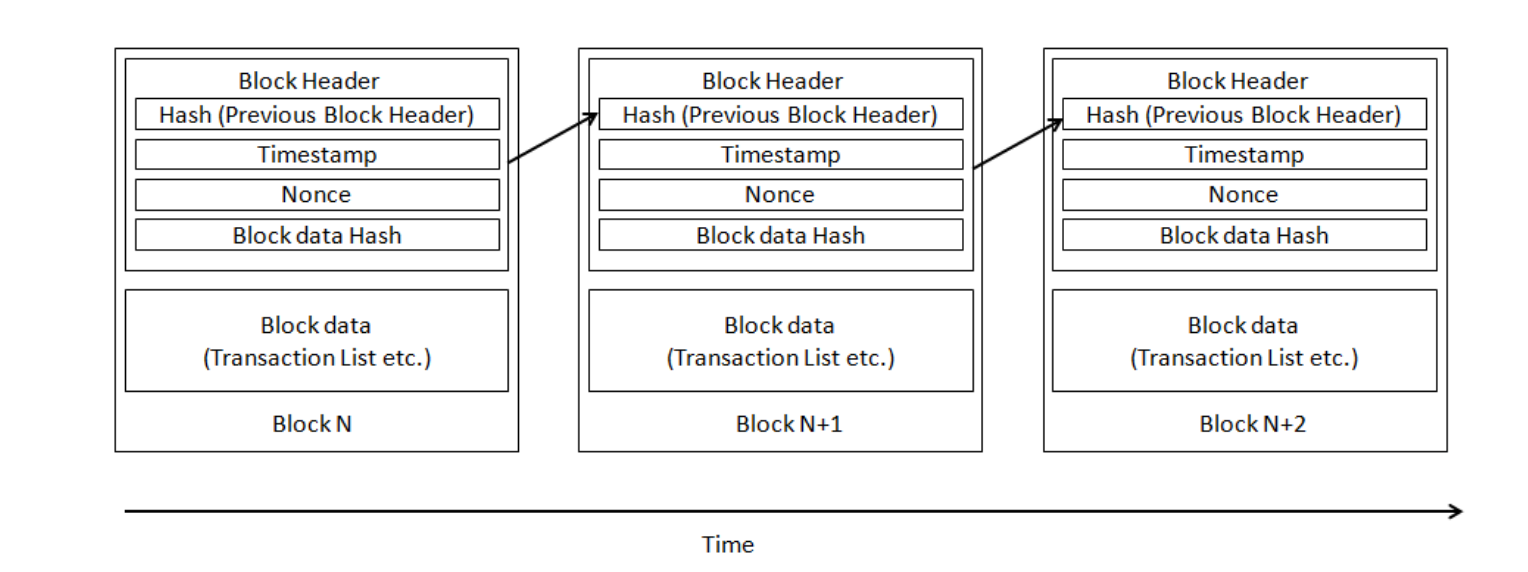
\includegraphics[width=1.95\textwidth]{images/chap01_BlockChain.png}
 		\end{minipage}
 		\caption[Generic chain og blocks]{[18740]}
 		
 		
 	\end{figure}
 	
 \end{center}
Blockchain has four main concept: \textit{P2P network:} node can interact with each other using private for sign transaction and public keys sre used as address that can be reachable on te network. \\
   \textit{Open distributed ledge}: It is like book containg all transactions that each node has the copy of data and there is no centrellized entity and any one can see assets and how much assets has each node.Therefor, they can decide about the validity of transactions.\\
   \textit{Schronization}: As, all node have one copy of ledger. Therefor, sycronization should prefome overall networks and by adddning new item or one new transaction should be performe in public and consensus needed to valid this transaction.\\
   \textit{Mining: }In the distributed ledger, all nodes can not receive transaction simultaneously. For adding new item in the blockchain, consensus of all nodes are needed. Thus there is need to prevent every onn node to add transaction into blockchain. Miners are the unique nodes that can add transaction to that chain. Miners attempts to validate the first transaction to add into chain.  
There are several distributed system based on consensus, but the one outstanding feature that makes blockchain  more prominent then the others is that :
 Only single record stores in each participant computer. This provides transparency of transaction. Whilst storing whole 
records over all networks of participating computer mitigate the probability of losing infrastructure.[2016 book 491]\\
And blockchain is the sole technology which fulfill such properties:\textit{(a)trustless}: There is no need to verify involved identities in transaction. \textit{(ii) Permissionless}: there is neither permission nor controlling for participants in network.   \textit{(iii)censorship resistant}: Anyone can trades on blockchain and just cryptographic algorithm governs the operation that entities(participants) can trust it.[50]


this feature and above reason make the block chain as powerful and most secure technology in commercial events over network.[50]

\begin{center}
	\begin{figure}[htb!]
		
		\begin{minipage}{0.55\linewidth}
			\centering
			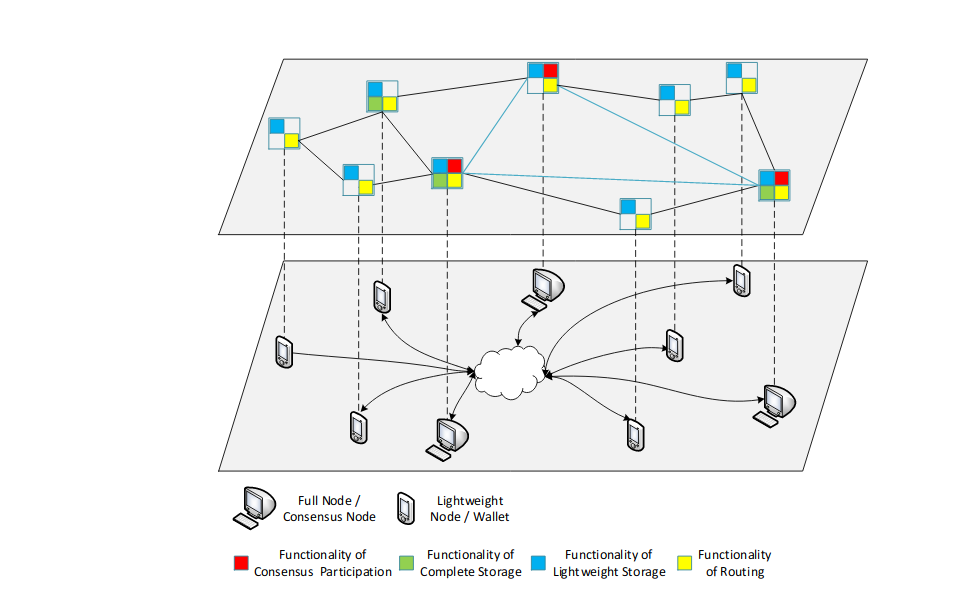
\includegraphics[width=1.95\textwidth]{images/chap01_P2P.png}
		\end{minipage}
		\caption[Permissionless blockchain network. The P2P links between consensus nodes are shown in blue.]{[60]}
		
		
	\end{figure}
	
\end{center}

\textbf{Permissionless / public Blockchain} This blockchain allows any0ne to join to network and create consensus such Bitcoin nd Ethereum. oin permissionless  blockchain any miner can create consensus mechnism such as proof of work, proof of stack to validate transaction. but as this mechanism is decentraliised the rate of validity of function and scalabilitiy is low.[30]

\textbf{Permissioned/ Private Blockchain}: this blockchain, only restricted  participant has right to validate transaction. Threfore, it provides better privacy and scalability. Unlike permissionless blockchain, this blockchain does not have  mining computation to reach the consenus because all participant are known in this network. [30]
\textbf{Privare Key/wallet}

\subsection{Bitcoin} 
The basic goal of blockchain technolgy is to ensure people form truthworthy and ligimacy of transactions. Blockchain initially used to enhance commercial transaction through currency called Bitcoin. \\
Bitcoin is the digital records or cryptocurrency that is accept by users involved in transaction. in fact, Bitcoin is the financial use cases of this powefull technology.[50]
Bitcoin is the list of blocks of transactions. Each block in blockchain is identifeid by hash algorithm on the top of the block.
Bitcoin is introduced by consensus mechanism of blockchain, it is well known implimentation of decentralized cryptocurrency.\\
Bitcoin is the limit of block, wherein each block is verified by hash algorithm using SHA256 cryptgraphic on the top of block. Each block encompass the hash of its parent (previous block) in the own header that refuse to it.
It forms block list wherein each block refers to previous block in the list name  genesis block[1]. Altering in block implies to create new blockon the top. Since, each block contains the hash of its parent creating new block is expensive and  needs proof of work that the miners allow the add new block.[1]

\subsection{Proof Of Work}
Is consensus algorithm in blockchain without any central algorithm that used to confirm transaction and add new block. With POW miners compete to complete its own transaction first into blockchain and get rewards(e.g: Bitcoin, Ether, ...).\\
Miners connected to blockchain and accomplish task validating transaction to add new block bc solving cryptographic puzzle[1].
TODO
\subsection{Mining}
Is an process if computation on the blockchain in order to verify and add block.[29]
TODO

\subsection{Merkler Tree}
all transactions are stored in tree structure wherein leafs contain transactions and internal node contain the hash of its sub tree and single root also contains the hash of two children  and represent top of tree. The purpose of bottom up hashing is that, if attacker attempts to create fake transaction into bottom of tree. This will change the node above and subsequently change the root. Thus altering the hash of block causing to register new block. Only the sequence of hash form root the leaf called the Merkler tree. [8a]   
\begin{center}
	\begin{figure}[htb!]
		
		\begin{minipage}{0.55\linewidth}
			\centering
			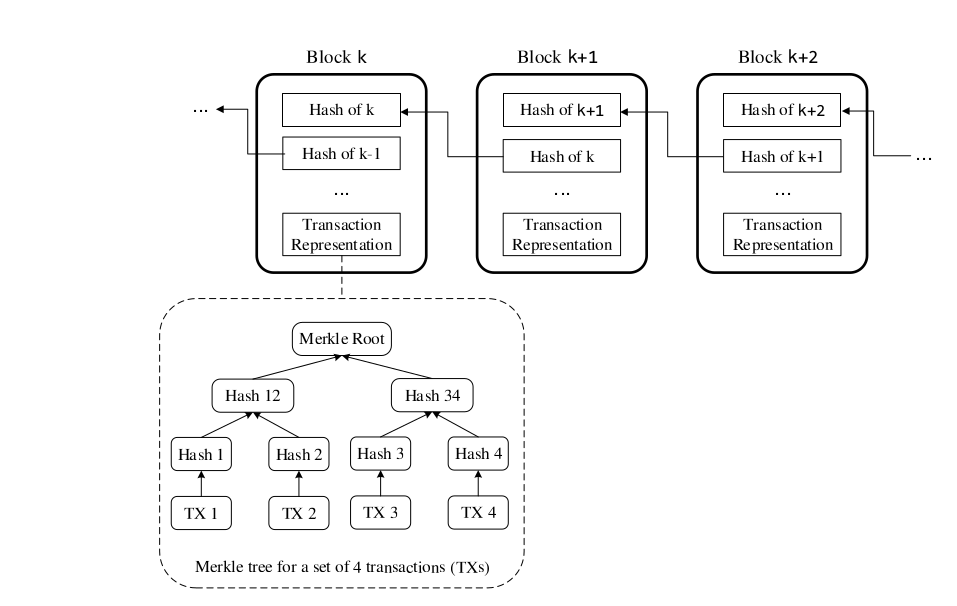
\includegraphics[width=1.85\textwidth]{images/chap01_Markler_tree.png}
		\end{minipage}
		\caption{Illustration of chain of blocks and  markler tree in single block}{[60]}
		
		
	\end{figure}
	
\end{center}

\subsection{Hash Function}
It is mathematicaly method to applay cyptografic(secret writting) function. hash function is deterministic means for an input produce same output each time. altering data generate the different output. 
According to Wikipedia, the security level of hash function has different properties: \\
\begin{itemize}
	
	\item {Pre-image resistance}: It s not easy, for initial input with /{h /}  hash value find the output value \{m\} , in a way that \{h = hash(m) \}
	
	\item {Second pre-image resistance}: it is not easy, for input \(m_1\)  find another input \(m_2\)   in way that \()hash(m_1)  = hash(m_2)\) and both have same result.
	\item {Collisio Resistance} : it is difficult to find two different input \(m_1  , m_2)\) that have same output in way that\( hash(m_1) = hash(m_2)\).\\
\end{itemize}
	Hash function used in blockchain and it is the most secure hashing algorithm is SHA256 which that provide the combination for an given input with 256 bit length. Using SHA 256 in blockchain makes to be impossible to dublicate hash because there are diverse combination of this input with this length and it requires huge amout of computaional works. That means thare are \( 2^ {256} \) hash values.
	
     \begin{center}
     	\begin{tabular}{c | c }
     	
     	 Input value  & SHA 256, message hash\\ 
     	 
        \hline
          1   &  6b86b273ff34fce19d6b804eff5a3f5747ada4eaa22f1d49c01e52ddb7875b4b \\
        \hline
     	  2    &   d4735e3a265e16eee03f59718b9b5d03019c07d8b6c51f90da3a666eec13ab35	\\
     	 \hline
     	 Blockchain & 625da44e4eaf58d61cf048d168aa6f5e492dea166d8bb54ec06c30de07db57e1 \\	
        \end{tabular}
        
     \end{center}


\subsection{Header} contains timetamp, nonce, previous hash, ...
\subsection{Nonce} it stands for \textit{number ued only once}. It is intger number and along with block data, number and previous hash use as input in SHA256 function to generate current block hash. We used this nonce to vary the hash of current block and without modifying  the data inside the block.the By the usage of nonce, miner can generate valid hash, adding first  own block into blockchain and get the reward.


\subsection{Transaction} transfer data (asset) between users, an transaction contains inforamtion such:\
- The recipents which message to send.
- Signiture of sender 
- A mount of ether to transfer
-Structure value, the maximum number of computational step that transaction is allowed to do 
- Gaspreice, fees that should pay.[29]

\subsection{Proof Of Stack} 

\subsection{Cryptographic hash functionn}
\section{Ethereumt}
Ethereum is the decentralized virtual machine based on block chain. Ethereum block chain stores codes of program and transaction data both on both on block chain. The code of contract is fed into block chain without address. Afterwards, the contract which already added to block chain and assigned address. As said before,the code of contract is unmodified, unlike contract's state that could be altered any time.
In Ethereum virtual machine, node or block besides adding the transaction to ledger, render contract codes and control the state in virtual machine.\\

TODO
Undoing smart contract etheruem ??
attack on ethereum smart contract.
\subsection{Security in Smart contract}

An  analysis  of  existing  smart  contracts  by  Bartoletti  andPompianu[7]shows that the Bitcoin and Ethereum platformmainly  focus  on  financial  contracts.  In  other  words,  mostsmart contract program code defines how assets (money) move.Therefore,  it  is  crucial  that  contract  execution  is  performedcorrectly.  The  direct  handling  of  assets  means  that  flawsare  more  likely  to  be  security  relevant  and  have  greaterdirect financial consequences than bugs in typical applications.Incidents, like the value overflow incident in Bitcoin [8], or theDAO hack [9] in Ethereum, caused a hard fork of the blockchain
to  nullify  the  malicious  transactions.  These  incidents  showthat  security  issues  have  been  used  for  fraudulent  purposesruthlessly in the past. A survey of possible attacks on Ethereumcontracts  was  published  by  Atzei  et  al.[10]and  lists  12vulnerabilities that are assigned by context to Solidity, the EVM,and blockchain peculiarities itself. Many of these vulnerabilitiescan be addressed by following best practices for writing securesmart contracts, which are scattered throughout the Ethereumcommunity [11,12] and different Ethereum blogs. Most bestpractices mainly contain information about typical pitfalls toavoid and the description of favourable design and problemapproaches. The latter being the focus of this paper in orderto collate smart contract security design patterns.[scsecurity]
\subsection{Vulnerabilities in Ethereum Smart Contracts}

Author in this section categorized the vulnerabilities in smart contracts into three classes(solidity, Ethereum virtual machine, blockchain):\\
\begin{center}
   \begin{tabular}{c |c }
   	\hline
   	    cal1 & cal2 \\
   	\hline
   	  \multirow{2}{4em}{Solidity} & Call to the unknown \\ & Gasless send \\ & Exception disorders  \\ & Type casts \\ & Reentrancy \\ & Keeping secrets \\
   	\hline 
   	  \multirow{2}{4em}{EVM}& Immutable bugs \\ & Ether lost in trasfer \\ & Stack size limit \\
   	\hline  
   	 \multirow{2}{4em}{Blockchain} & Unpredictable state \\ & Generating randomness \\ & Time constraints \\
   	\hline
   \end{tabular}	 
 
\end{center}
\textbf{- Call to Unknown:} One invokes the function and transfer the ether to the counterpart. If there is no signature in the given address, then the fallback function is executed.\\ 
for example: In the contract \textit{Alice} and  \textit{Bob}:\\
 Alice has \textbf
{Ping} function and Bob invokes the Alice contract (\textbf{ping} function) via direct call. If there is any mistype in calling function such as \textit{int} instead of \textit{Uint} call to the \textbf{ping} return fallback function. \\

\texttt{\color{red}contract \color{black}Alice \{ \color{red}function \color{black}ping (\color{red} uint \color{black}) \color{red}returns \color{black}( \color{red}uint \color{black}) ; \} }\\
\texttt{\color{red}contract \color{black}Bob
	\{ \color{red}function \color{black}pong (Alice c) \{c.ping (42); \} \}}
\\
Or in another contract: \\
\texttt{c.\color{red}call . value \color{black}(amount)(bytes4(sha3("ping(uint256)")),n); }\\
function \textbf{ping} in contract \textbf{c}: called function is identified by hash signature.\\
\textbf{amount } is the much of \textit{wei} that is to transfer to contarct \textbf{c}.\\
\textbf{n}  is parameter in \textbf{ c}. If the function with this signature does not exist in the contract the fallback function is executed.  
\\

\textbf{- Exception disorder: } this is occurred in situation such as: executation run out of gas, call stack reaches to its limit and \textit{throw} commend is executed.
For instance in this contract:\\
\texttt{\color{red}contract \color{black}Alice \{ \color{red}function \color{black}ping (\color{red} uint \color{black}) \color{red}returns \color{black}( \color{red}uint \color{black}) ; \}}\\
 \texttt{ \color{red}contract \color{black}Bob
 	\{\color{red} uint \color{black} x=0;
 	\\ \color{red}function \color{black}pong ( Alice c ) \{ x= 1; c.ping (42); x=2; \} \}}\\
 
 There are two possibility of \textit{call }function: 
 \begin{itemize}[label={},leftmargin=12.5mm]
  \item User invokes Bob function, therefore, \textbf{ping} throw exeption and execution stops. Side effect of all transactions are reverted and \(x=0\) after transaction.
  \item  Bob invokes \textbf{Ping } via call, Only side effect of invocation reverted, call returns fail, execution continue and \(x=2\)  after transaction.
 \end{itemize}
\textbf{Gasless send: }\textbf{send} function , transfer ether to contract. This function compiled the same way of \textit{call }function without signature and returns \textit{out of gas} exception.\\
Assume \textit{call} has no signature, so it invokes \textit{callee's } fallbac  function. However  the upper bound of unit of gas is 2300 that is avaiable to \textit{callee } and is executable.

\begin{multicols}{2}
	\texttt{
		\color{black} 1 -\color{red}contract \color{black}C \{\\
		\color{red}function \color{black}pay(\color{red}uint \color{black}n, \color{red}address \color{black}d) \{\\
		d.send(n) ;\\
		    \hspace*{4mm}\}\\
		\}}
	
	 
	\columnbreak
	
	
	\texttt{\color{black} 2 - \color{red}contract \color{black}D1 \{\\
			\color{red}uint public \color{black}count = 0;\\
			\color{red}function \color{black}() \{ count ++; \}\\
	       \}
		\color{red}contract \color{black}D2 \{ \color{red}function \color{black}() \{\} \}}
	 
\end{multicols}

\textbf{Type casts}
\textbf{Reentrancy}
\textbf{Keeping secrets}
\textbf{Immutable bugs}
\textbf{Ether lost in transfer}
\textbf{Stack size limit}
\textbf{Unpredictable state}
\textbf{Generating randomness}
\textbf{Time constraints}

\chapter{Blockchain as the Infrastructure of Semantic Web}
Distributed ledger is increasingly used to represent transactions between multiple parties throughout the world. It is difficult to search for specific information in distributed ledger without an index. Therefore, indexing data in the distributed ledger is a requirement that provides the ability to search across multiple ledgers, enhancing the power and usability of this system as well \cite{Third}.
\section{Distributed Ledgers and Indexing}
A distributed ledger based on a blockchain does not have central control. Blockchains are organized into multiple blocks the initial block is created manually and the other blocks are added by some consensus process between nodes.
Ethereum smart contract provides the possibility to control automatically what happens with cryptocurrency on the blockchain without involving untrusted external sources. Ethereum smart contracts have an account that can normally store, update, or make a function with the input and output.
As smart contracts are time-ordered where data are stored in blocks,  requires the data to index. Indexing the smart contract gives us the capability to access the data, search, analyze services on the distributed ledger, and expose them to outside the world for more interactions.
There are different levels of indexing smart contracts: Basic level is the fundamental level for the next step. It indexes basic entities such as accounts, blocks related to distributed levels, and data can be stored or retrieved here. At the functional level, smart contracts contain a lot of functional interfaces that depict the other functionality of platforms such as Ethereum \cite{Third}. 

\subsection{Why do we use Ontology for Blockchain?}
Generally, Blockchain is the distributed database that is replicated over all nodes as a cloud computing architecture. These databases are distributed across multiple organizations. Thus, data should have a common interpretation to be understandable for organizations. Interpretations are applicable via formal specification that enables verification and inference within software and applications executed on the network. \\
This is where ontology plays the main role to ensure a common interpretation of data in the shared database among different enterprises.
blockchain as a modeling form used a different type of ontology: \\
\\
\textbf{\textit{Informal/Semi ontology}} facilitates search and enhances a better understanding of the business process for developing and applying on the blockchain.\\
\\
\textbf{\textit{Formal ontology}} helps the formal specification to automate inference and verify the operation of the blockchain. In other words, blockchain modeling based on formal ontology can help the development of smart contracts to execute on the blockchain.\\
\\
Also, we can use ontology to capture data within blockchain: On one hand, It facilitates a better understanding of blockchain concepts for humans. On the other hand, enables interlinking with other linked data to convey deductions and formal reasoning \cite{Kim}.\\
Vocabulary used within ontology increases the transparency of transactions by describing the transaction in the context of linked data and facilitating the graphical representation of the location of such transactions. Thus, it increases also the capability of analysis by users \cite{Kim}.

\begin{center}
	
	
	\begin{figure}[htb!]
		
		\begin{minipage}{0.55\linewidth}
			\centering
			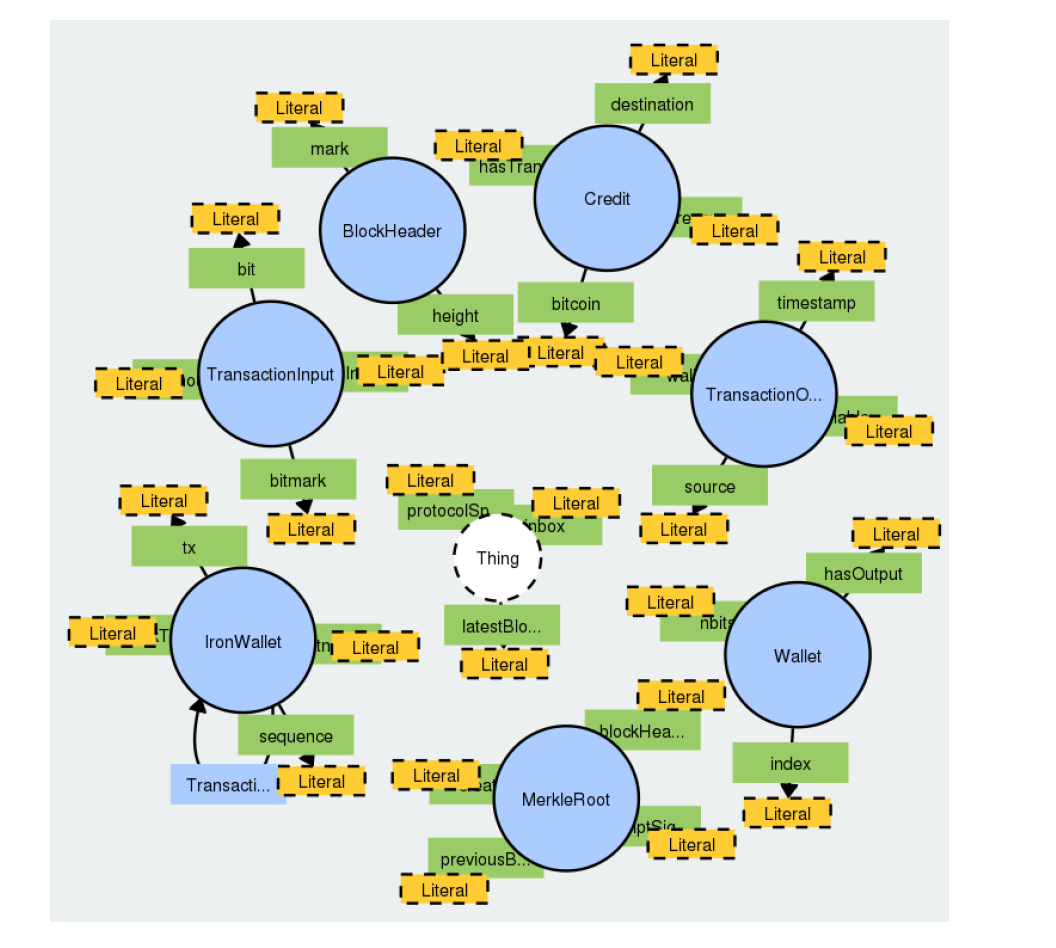
\includegraphics[width=1.65\textwidth]{images/chap02_diagram_ontology.png}
		\end{minipage}
		\caption[Illustration of ontology diagram]{Illustration of ontology diagram \cite{Matthew}}
		
		
	\end{figure}
	
\end{center}

\subsection{Linked Data}
According to Tim Berbers-Lee et al.\cite{Tim}, 'Linked Data is about using the Web to create typed links between data
from different sources'. When information
is presented as Linked Data, other related information can be easily retrieved and new information also can be easily linked to it. \textit{Berners-Lee} described four rules for linked data:\\
\textbf{- URIs} (Uniform Resource identifier) as names.\\ 
\textbf{- HTTP} to search for names.\\
\textbf{- (SPARQL, RDF)}  when a user searches for something, provides related information.\\
\textbf{- Link} to other URLs to provide more information \cite{Hector}.\\

\begin{center}
	\begin{figure}[htb!]
		
		\begin{minipage}{0.55\linewidth}
			\centering
			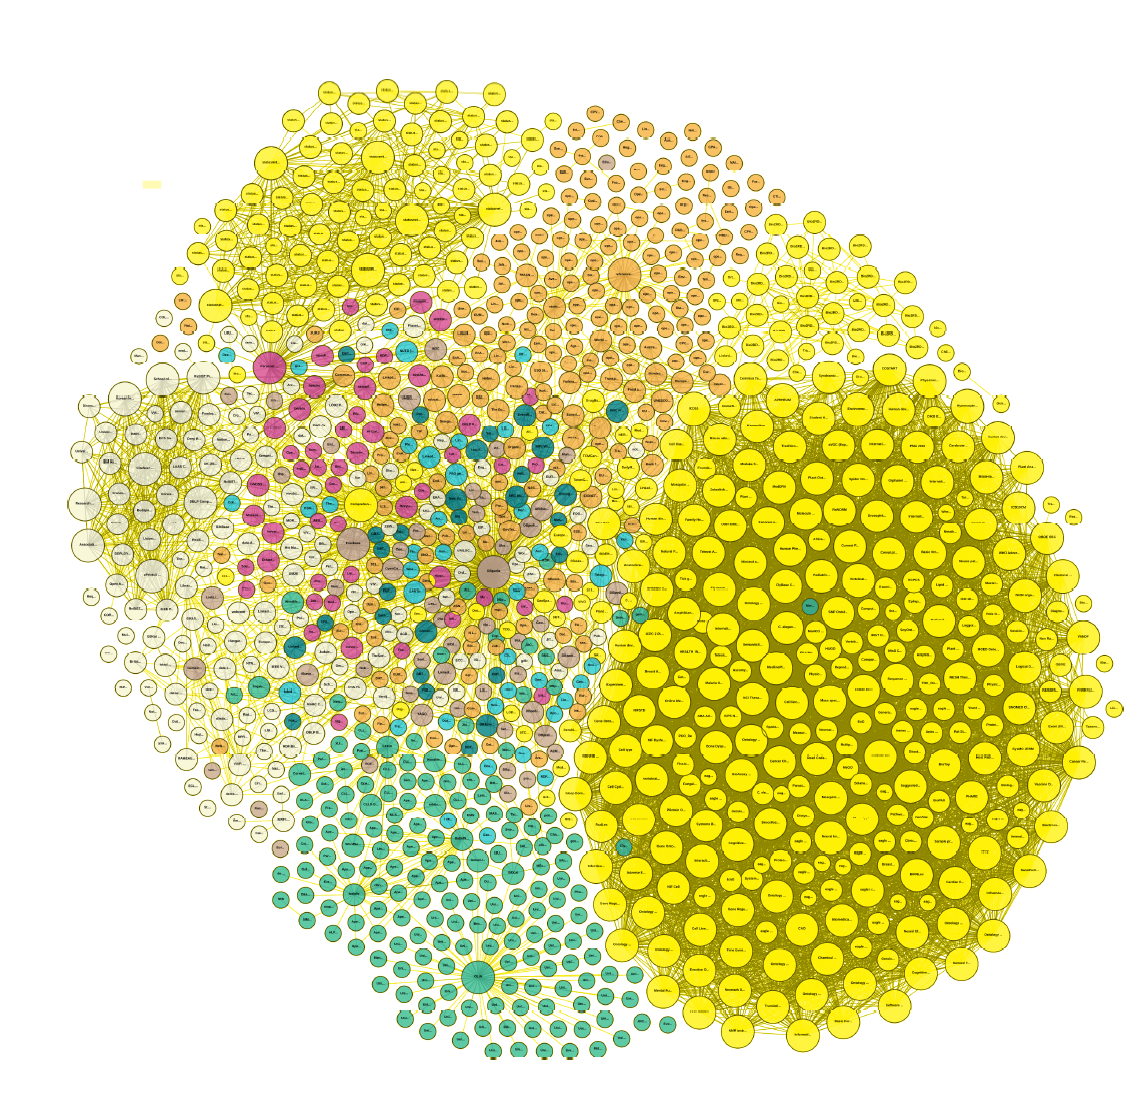
\includegraphics[width=1.55\textwidth]{images/chap02_LinkData.png}
		\end{minipage}
		\caption[Linked data diagram]{Linked data diagram \cite{Hector}}
		
		
	\end{figure}
	
\end{center}
\subsection{RDF}
The Resource Description Framework (RDF) is a family of W3C specifications. RDF is used to describe and model information. It describes a subject that predicts an object is called a triple.
i) Subjects that RDF expressions describe them.
ii) predict is specific properties, attributes, or relation to describe a resource.
iii) The object is the name of a property or value.
We can build a graph based on these three objects \cite{Hector}.

\subsection{SPARQL}
According to Wikipedia definition: It is a semantic query language for a dataset that makes us able to retrieve and modify data stored in RDF format known as triple. SPARQL can query the one, two, or all elements of triples.    

\subsection{OWL (Ontology Web Language) }
Ontology Web Language is made to represent knowledge about things and the relations among them. OWL is a computational logic-based language, which means the language modeled in OWL can operate in a computer program like negation, intersection, and so on \cite{Hector}.
\subsection{Web 3.0}
Evolution and interaction of people on the Internet are classified based on three technologies:\\
\textit{Web 1.0} is known as \textit{web of document} is the earliest website with the basic capability of linking to other websites.\\
\textit{Web 2.0} known as \textit{web of data} has the capability of providing space for users to collaborate with content creation or modification.\\
\textit{Web 3.0} is strengthened by the semantic web, where people have access to linked information on the web. But newly, with the arrival of distributed technology like blockchain, and Ethereum which get used by Web 3.0, this is a new focus on this \cite{Chhetri}.
\section{Vocabularies}
\subsection{Vocabulary in Distributed Ledger}

Generating linked data requires to use of a standard ontology or vocabulary to explain the blockchain concepts. Interfaces between distributed ledgers and the Semantic Web are still in an early stage. Some systems define such vocabulary such as FlexLedger, EthOn, BLONDiE \cite{Third}.\\
\\
\textbf{\textit{FlexLedger}} describes HTTP interfaces to blockchains, with a standard vocabulary and responses of these interfaces. FLexLedger is a protocol for decentralized ledger and graph data model which represents ledger creation, querying, and data model using JSON-LD. However, FlexLedger does not have explicit vocabulary about ontology nor has concrete ontology for itself. \\
It is striking to say that the FlexLedger is not suitable to implement in some graph models like graph chain because in FlexLedger meta and the content data are stored together in the same graph whereas the GraphChain blocks’ content is stored outside the blockchain a separate graph \cite{Sopek}.\\
\\
\textbf{\textit{EthOn}} is an OWl ontology that describes blockchain classes such as \textit{"blocks, accounts, message", "state"} and relations such \textit{"has parent block"} \cite{Rashid}. 
\begin{center}
	
	\begin{figure}[htb!]
		
		\begin{minipage}{0.50\linewidth}
			\centering
			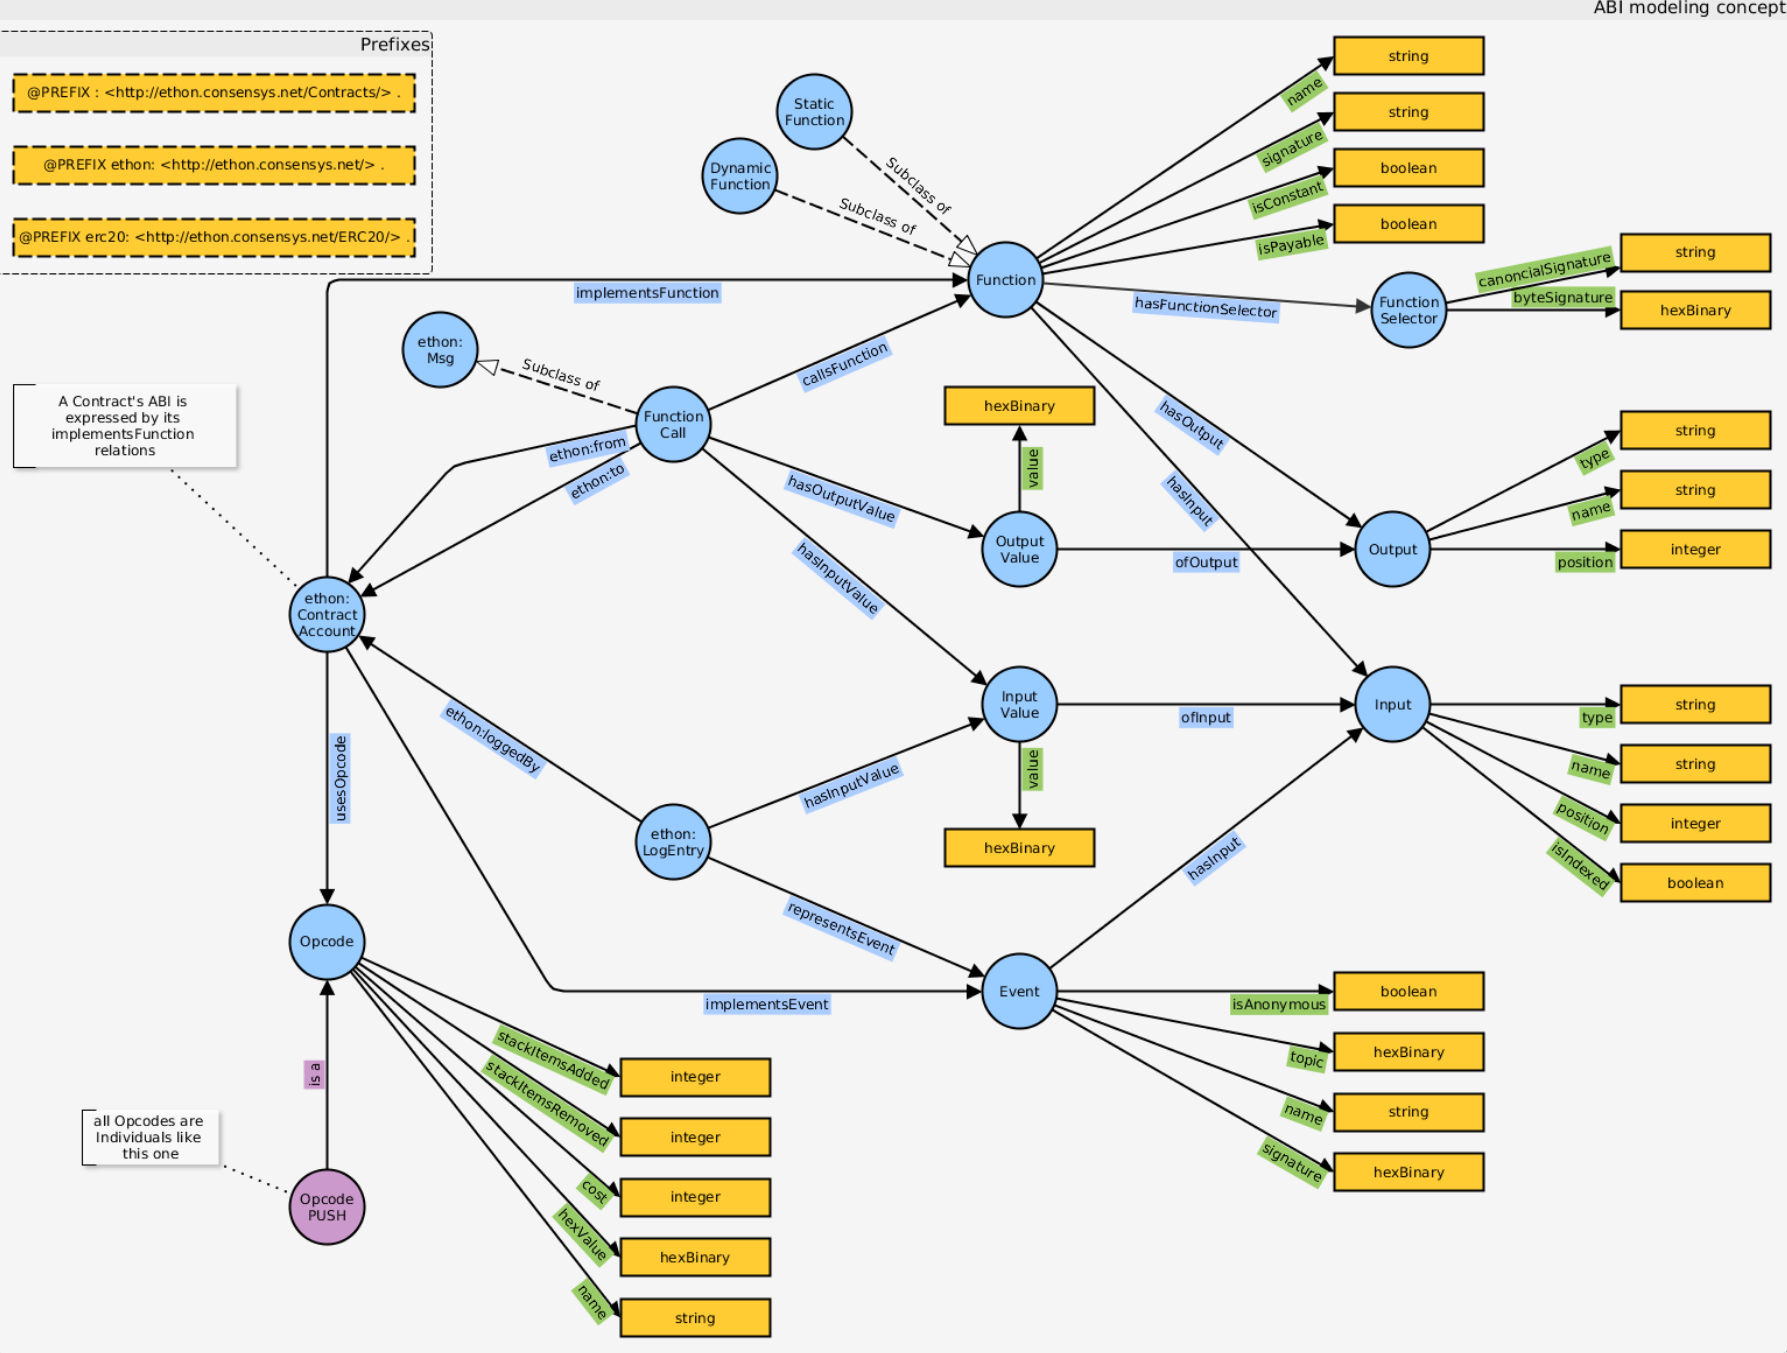
\includegraphics[width=1.80\textwidth]{images/chap2_EthOnContract.png}
		\end{minipage}
		\caption[EthOn classes]{EthOn contract model(blue arrow is object properties, green arrow is data properties, purple circle is instance and blue one is class) \cite{Rashid}}
		
	\end{figure}
	
	\begin{figure}[htb!]
		
		\begin{minipage}{0.55\linewidth}
			\centering
			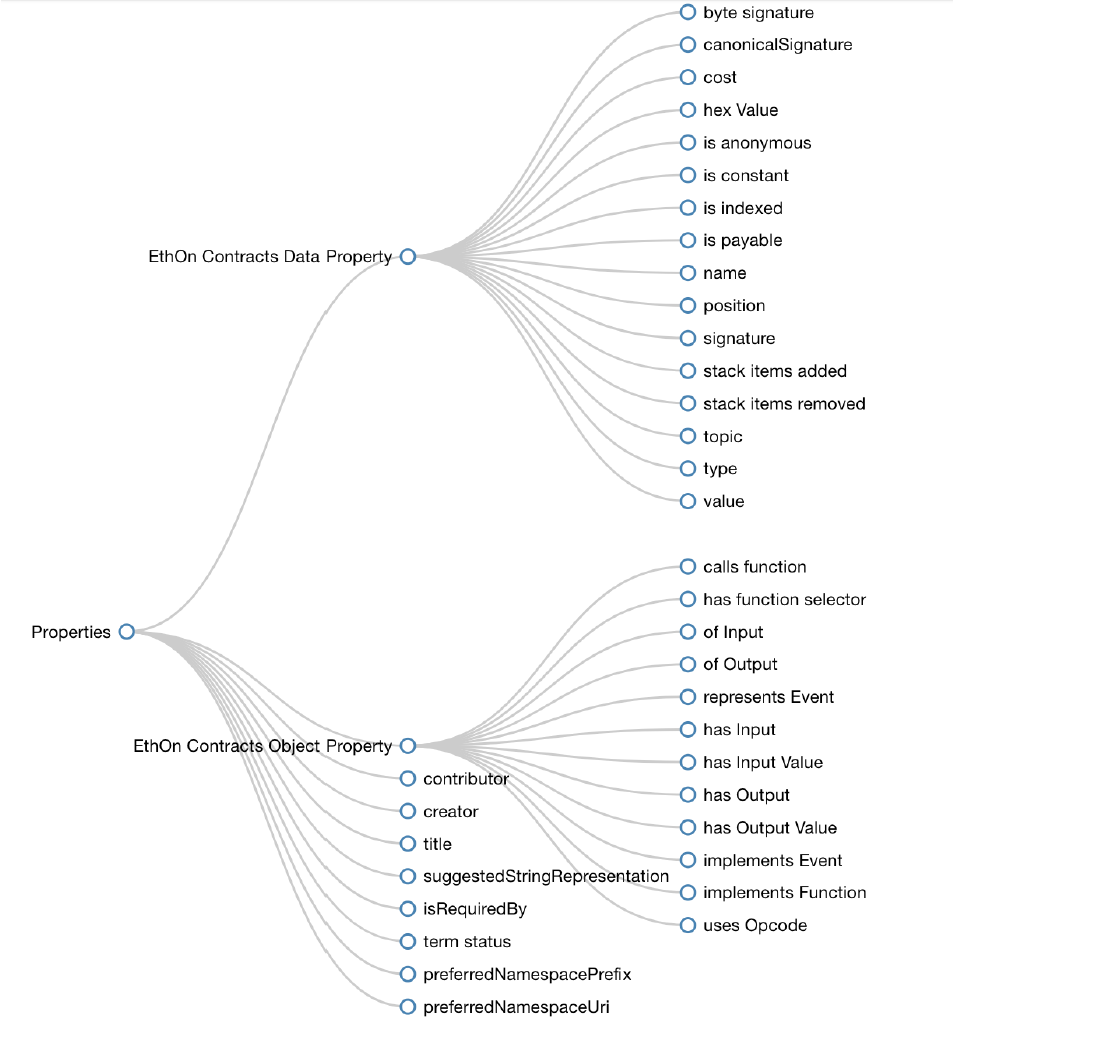
\includegraphics[width=1.65\textwidth]{images/chap02_EthOn_Properties.png}
		\end{minipage}
		\caption[EthOn Properties]{EthOn classes \cite{Rashid}}
		
		
	\end{figure}
	
\end{center}
\textbf{\textit{BLONDiE (Blockchain Ontology with Dynamic Extensibility)}} is another OWL ontology for describing the Blockchain structure like EthOn. But, it is more generic than EthOn. For example, EthOn and BLONDiE both defined some terms such as 'account', 'block', and 'transaction', and some attributes such as 'transaction payload' or 'miner address'. BLONDiE defines some other concepts for different Blockchain such as 'BitcoinBlockHeader' and 'EthereumBlockHeader' as subclasses of 'BlockHeader'. At the moment, BLONDiE supports two cryptocurrencies like bitcoin and Ethereum where all links and relations between objects and attributes represent in RDF (Resource Description Framework) \cite{Third}.
\begin{center}
	\begin{figure}[htb!]
		
		\begin{minipage}{0.55\linewidth}
			\centering
			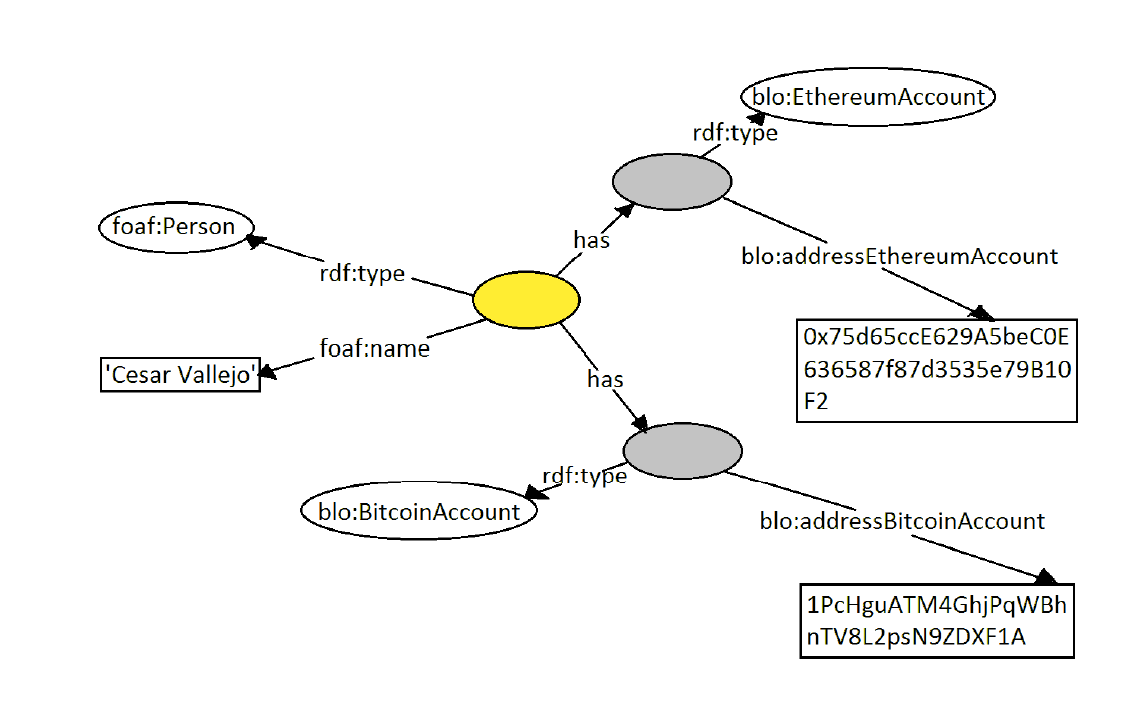
\includegraphics[width=1.75\textwidth]{images/chap02_BLONDiE.png}
		\end{minipage}
		\caption[BLONDiE]{BLONDiE usage example \cite{Hector}}
		
		
	\end{figure}
	
\end{center}
\subsection{Vocabulary in Smart Contracts}
As mentioned earlier, EthOn and BLONDiE are both similar concepts that can be used for smart contracts. There are many works on semantic annotation of the web and HTTP APIs which may enable us to annotate smart contracts as well. However, the contracts are not Web API and implementation may differ but the main concept does not differ. In other words, the vocabularies used to annotate web services, are used to annotate smart contracts too. It seems that the combination of a distributed ledger with the smart contract and web service due to profitability becomes common \cite{Third}.

\section{Semantify Blockchain}
\subsection{Semantic Blockchain}
With increasing the use of blockchain technology recently, the need for semantic reasoning on the distributed ledger is on the increase as well. The blockchain is the best platform to utilize semantic web principles in this technology and add a new trusted property to a dataset. 
Using semantic web technology on the blockchain is a novel idea and the way how to apply this technology in blockchain and smart contracts is also a controversial issue.\\
There are some \textbf{definition of semantic blockchain:}\\ 
\textit{- Semantic blockchain is the representation of stored data on distributed ledger using linked data. }\\
\textit{- Semantic blockchain is the applying semantic web standard on the blockchain that these standards are based on RDF \cite{Hector}.}

\subsection{Semantification Process}
Semantic blockchain or semantic distributed ledger affects the industrial world and subsequently, the result leads to the start development of new applications and frameworks to combine two worlds:
these are some ways to samantify blockchain:\\
\textbf{-} Mapping the blockchain data to RDF making usage of vocabulary, ontology, and so on.\\
\textbf{-} Storage of data in a blockchain is expensive, The only way is to store the hashing point to the data set in the blockchain and then share RDF on the blockchain. \\
\textbf{-} Creating semantic blockchain that exchanges internal data protocol in RDF format \cite{Hector}. \\

\subsection{Semantic Ontology Mapping using BLONDiE} 
To generate RDF, it needs to map the basic blockchain entities to relevant semantic web terms, concepts, and ontology. To make the query more efficient, BLONDiE is extended in two ways: Firstly, records relating to both block and transactions have been
augmented with an attribute for the hash of each entity. Secondly, records relating to the transactions have been augmented with links to entities like blocks or smart contracts.\\
Blockchain stores just a binary form of each contract with metadata.   
To interact with the contract Application Binary (ABI) Interface specification is required. This specification is in the form of JSON and is created when a smart contract is compiled and stored in the blockchain. The ABI determines all functions of contracts and descriptions about input, and output parameters for each contract \cite{Third}.

\begin{center}
	\begin{figure}[htb!]
		
		\begin{minipage}{0.45\linewidth}
			\centering
			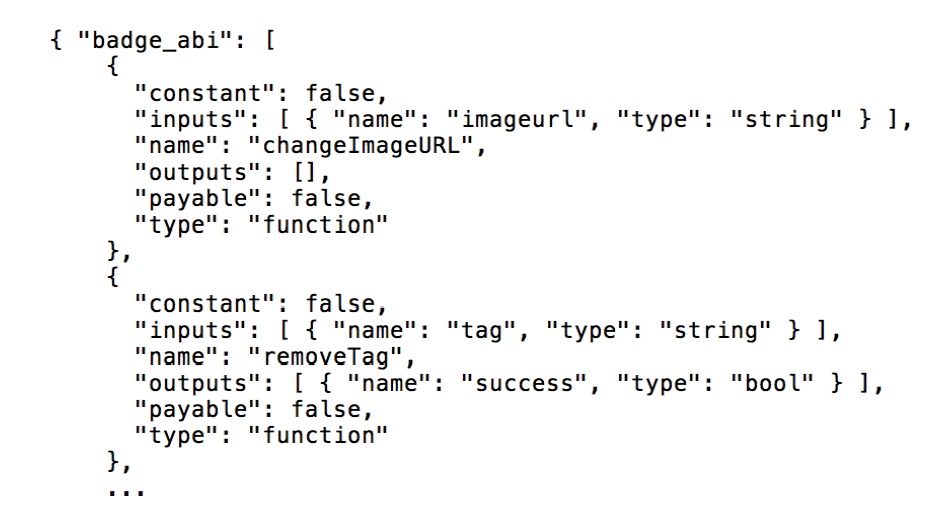
\includegraphics[width=1.95\textwidth]{images/chap02_SmartContract_ABI.png}
		\end{minipage}
		\caption[Smart contract ABI]{Smart contract ABI}
		
	\end{figure}
	
\end{center}
\chapter{DALICC}
\section{DALICC}
According to [], DALICC stands for Data Licenses Clearance Center. It is software framework that helps people to legally secure data from third party and help to detect licensing conflicts and reducing the costs of rights clearance by enabling automated clearance right in creation of derivative works. 
\subsection{DALICC Requirements}
The following requirements would be addressed by DALICC framework:\\
\begin{itemize}
	\item \textit{Tackling license heterogeneity:} \\
	It is possible to combine the various contents which having the same license with different names. But that would be much difficult to license the resultant of the combined contents. To solve this issue, DALICC provides set of machine-readable representation of licenses that allow to compare licenses to each other to identify the equivalent licenses. It guides the user to possible conflicts of various combined licenses.
	\item \textit{Tackling REL heterogeneity:} \\
	Combing licenses are simple, if they are express through the same RED. But, it is difficult to compare licenses have been represented by different RELs.\\
	DALICC resolve this problem, by representing RELs based on semantic web, map the terms to each other. It will represent exiting RELs based on  W3C-approved standards, thus allow mapping between various RELs to be created.
	\item \textit{Compatibility check, conflict detection and neutrality of the rules:} \\
	It is difficult to be sure, if the meaning of the different terms in semantic are aligned. This problems result from indicating the classes, instances and properties which can not be handled just by mapping.\\
	This is where DALICC comes to play and helps user with a workflow that define the usage context, then gathering additional information to detect conflicts and ambiguous concepts. Based on this information, DALICC make reasoning over the set of licenses and infers the instruction to user how to process with license processing.\\
	\item \textit{Legal validity of representations and machine recommendations:} \\
	According to Anna Fensel\cite{Anna}, The semantic complexity of licensing issues means that the semantics of RELs must be clearly aligned within the specific application scenario. This includes a correct interpretation of the various national legislations according to the country of origin of a jurisdiction (i.e. German Urheberrecht vs. US copyright), the resolution of problems that are derived from multilinguality and the consideration of existing case law in the resolution of licensing conflicts.\cite{Anna}\\
	To solve this problem, DALICC will check the legal validity of machine-readable license and compatibility of reasoning engine output with law. DALICC output will be testes against law and checked the semantic precision of derived from different language and adjusted them.
	
\end{itemize}
\subsection{DALICC Software Architecture}
To address the above challenges DALICC framework consist of four components:\\
\begin{itemize}
	\item \textbf{License composer} is tools that allowed the license to be created from set of questions which are mapped to ODRL, ccREL and the DALICC vocabularies and concepts.
	\item \textbf{License library} is a repository that represents licenses in machine-readable format , the former as ORDL policies and the letters as plain text.
	\item \textbf{License annotator} allows to attache license to dataset, either by choosing available licenses in license library or create new license using license composer.
	\item \textbf{License negotiator} as main component in DALICC framework that checks the license compatibility and support license conflicts by detecting equivalence license having various names.
\end{itemize}

\chapter{Implementation: DApp}
DApp is often described as P2P, trustless with a special characteristic that there is not a single server to control it. DApp includes at least one User interface or frontend that could be a Mobile app, Desktop application installed on a computer.\\
The data relating to the application could be provided by a single group or company or may provide by end users themselves. Finally, it involved some kind of data manipulation. \\
DApp uses the ethereum as backend of its data storage and processing using smart contracts. The user interface of DApp is usually like traditional websites but is one website plus one or multiple smart contracts.

\begin{center}
	
	\begin{figure}[htb!]
		
		\begin{minipage}{0.75\linewidth}
			
			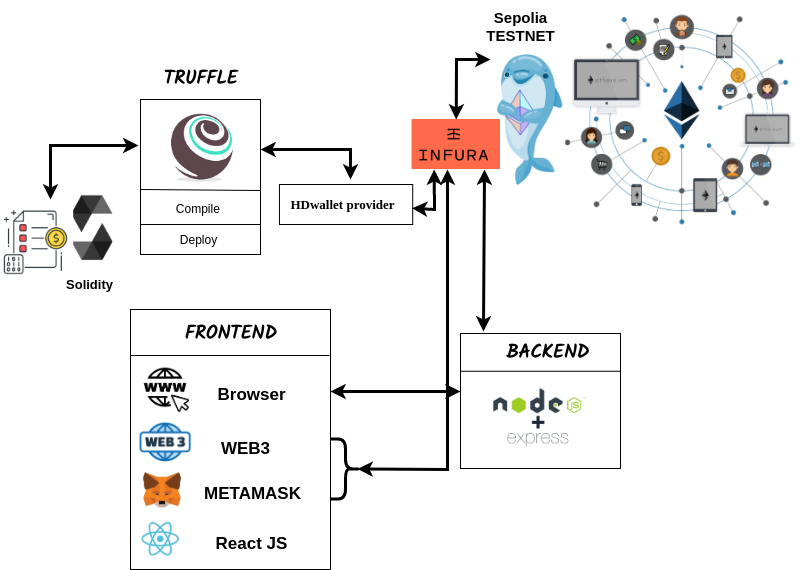
\includegraphics[width=1.45\textwidth]{images/chap03_dapp.png}
		\end{minipage}
		\caption{DApp infrastructure}
		
	\end{figure}
	
\end{center}

\section{DApp and Ethereum Blockchain}
The benefit of using the Ethereum blockchain in DApps are as follows:
 \begin{itemize}
     \item 1- The user can see what is going on before submitting any data.
     \item 2- Once the user has interaction, no one can temper or delete data.
     \item 3- The user of the application can directly participate in application management.
 \end{itemize}
\section{Project Concepts}

In this section, we focused on the requirements that we need to address in our application.
\\
\subsection{Contract and Ontology Specification}
Here, it is explained some terms related to smart contracts and the ontology of our application. And we needed them as the primary requirement to build up this dApp.
\begin{itemize}
	\item \textbf{Definition 1 (Owner)} is the address of deployed contract or transaction to the blockchain. That is the first person who interacts with the contract. In this case, the owner can change her/his license of the file.\\
	\item \textbf{Definition 2 (Non-owner)} is the another user that make not action. In this case, can retrieve license information related to specific files.\\
	\item \textbf{Definition 3 (Licensor)} is the address currently interact with smart contract. In this case, can license his/her file.\\ 
	\item \textbf{Definition 4 (Semantic mappings)}: As we do not have the authority to change stored data on the Ethereum blockchain, one idea is to create a template to have a semantic view of the blockchain.
	To reach this purpose, we need a mapping between stored transaction data in the blockchain and transaction concepts defined as ontology, then make a query on produced data from this mapping. This process consists of three following requirements:
	
	\begin{itemize}
		\item \textit{Transaction Schema} are actually some attributes resulted from web3.eth functions that EhtOn data properties would be mapped to.
		\item \textit{Transaction Triple template} defines for the relationship between concepts(block or transaction) and properties. It is known as 'Subject predicts Object' that Subject is the web3.eth properties, predict known as EthOn ontology predictor(data properties) and Object (web3.eth properties) is a place that would be replaced by the transaction schema on the mapping. 
		\item \textit{Triplize} is the function that generates data in RDF format by creating a mapping between the two above parameters as input. 
	\end{itemize} 
     \item \textbf{Definition 5 (Prefix)} name is the label or local part separated with ':' and is the abbreviation of terms that referenced resources explicitly. According to Wikipedia, Prefixes are declared on the top of the SPARQL query and our triple template, so that the statements can reference to.\\
     \textbf{Definition 6 (Triple)} defined in Wikipedia as a statement with three entities that codifies semantic data in the form of \textit{Subject-predict-Object} expressions.\\
\end{itemize}
\subsection{Technology Usage}
\textbf{DApp} \\
It is a type of open-source smart contract application that runs on a decentralized peer-to-peer network rather than a centralized server. It allows users to transparently execute a transaction on a distributed network. \\
DApp is similar to centralized apps, as they use frontend and backend. But the backend's app is supported by a centralized server or database. And Backend's DApp runs on a decentralized p2p network and is supported by smart contracts which store on the Ethereum blockchain.\\
\\
\textbf{Decentralized application characteristic:}\\
	\textit{Open Source}: all the required are decided on a census of all available users on a network.\\
	\textit{Decentralized Storage}: data is stored on decentralized blocks.\\
	\textit{Validation}: As the application runs on blockchain. They offer validation of data using cryptographic tokens which are needed for the network. \\
 \\
\textbf{Ethereum} \\
it is explained in section 1.4.\\
\\
\textbf{Solidity} \\
it is explained in section 1.5.5.\\
\\
\textbf{SHA3-256} \\It is explained in section 1.5.3.
\textit{message} is the additional input parameter in text type\cite{fips}.\\
\textbf{Java Script Tools} 
\begin{itemize}
  \item \texttt{Truffle} is the smart contract development tools and testing network for blockchain applications and supports developers who are looking to build their dApp, etc. \\
 Truffle offers some different features: \\
 \textit{- Smart contract Managing}: truffle helps to Manage artifacts of smart contracts used in dApp and supports library linking, deploying, and some other Ethereum dApps. \\
 \hspace{3cm} \textit{- Contract testing system}: Truffle helps developers construct smart contract testing systems for all their contracts. \\
 \textit{- Network management} helps developers by managing their artifacts. \\
 \textit{- Truffle console} allows the developer to access all truffle commands and built contracts \footnote{https://moralis.io/truffle-explained-what-is-the-truffle-suite}.
\\
\item \texttt{React. js} is an open-source JavaScript framework which used as a frontend. In react, a developer builds a web application by using reusable individual components that are assembled from an application's whole user interface.\\
React has the advantage of providing a feature that combines the speed of JavaScript with a more efficient method of managing DOM to render web pages faster and create more responsive web application \footnote{https://blog.hubspot.com/website/react-js}.\\
\item \texttt{crypto. js} is the JavaScript library that performs data encryption and decryption. It is a collection of standard algorithms including SHA3-256 \footnote{{https://github.com/jakubzapletal/crypto-js}}.
\item \texttt{Web3.js} helps developer to connect to Ethereum blockchain. It is a collection of libraries that allows developers to perform some actions like sending ether, checking data from smart contracts, and creating smart contracts \footnote{https://www.datastax.com/guides/what-is-web3.js}.\\
\item \texttt{axios} provides the HTTP requests from the browser and handles request/response data \footnote{https://axios-http.com/docs/intro}. \\
\item \texttt{HDwallet provider} is a package to help the developer to connect to the network. It is easy to configure the connection network to the Ethereum blockchain through \textit{infura}. This provider is used by Truffle when we deploy the contract. In addition, meta mask providers are also used when we want to interact with the contract in the browser.\\
HDwallet provider provides a custom URL: 'http://127.0.0.1:7545'. This will spawn a development blockchain locally on port 7545 \footnote{https://github.com/trufflesuite/truffle-hdwallet-provider}. \\
\item \texttt{Express.js} is node.js framework for authority dApp. It provides HTTP methods (GET, POST) to call functions for particular URL routes \footnote{https://www.simplilearn.com/tutorials/nodejs-tutorial/what-is-express-js}. \\ 
When we run dApp, we have an HTTP server located on port 3000. \\
\item \texttt{FS} provides some functionality to interact with the file system, mostly used functions like: \textit{readFileSync}, \textit{writeFileSync} and \textit{appendFileSync} \footnote{https://blog.risingstack.com/fs-module-in-node-js/}. \\
\end{itemize}

\textbf{Semantic Web Tools}\\
\begin{itemize}
	\item \textit{EthOn Ontology} is semantic view of ethereum blockchain. It encompasses different classes and relations to cover different concepts of Ethereum like blocks, transactions, and messages to formalize RDF triple. We used classes and properties related to transaction concepts as a template to model our transaction to DALICC \footnote{https://axios-http.com/docs/intro}.
	\item \textit{SPARQL query} is defined in the section 2.1.4.
	\item \textit{Command-Line SPARQL with Jena} is a utility of Apache Jena that runs queries on remote SPARQL endpoint or RDF files that would be lo located on a local computer or web. We used the command as follows:\\
	 - Using Command line : \textit{sparql --data rdfFile --query sparqlFile}
	
\end{itemize}
\textbf{Ethereum Tools}

\begin{itemize}
\item \textit{Infura}, According to the internet definition, a web3 backend and infrastructure-as-a-Service (IaaS) provider offers a range of tools to help the developer to build dApp to connect to the Ethereum blockchain.\\
\item \textit{Metamask Wallet} Metamask is a wallet used to interact with the Ethereum blockchain. It allows users to connect network through a browser extension or mobile app. Metamask wallet, including all accounts, each account has its private key \footnote{https://originstamp.com/blog/metamask-what-is-it-and-how-does-it-work/}.\\
\item \textit{Faucet(ETH faucet)} is the platform that gives some test tokens to a user to test smart contracts or send transactions before deploying them to the main net. \\
\item \textit{Testnets} are the test blockchain networks that perform similarly to the main blockchain (mainnet). This allows developers to execute their contracts on test blockchain freely \footnote{https://blog.infura.io/post/introducing-infuras-eth-testnet-faucet-get-0-5-eth-daily-to-test-your-dapps}.\\
Infura's new testnet faucet is Sepolia ETH which provides the most reliable and high-volume faucets for developers. \\
\item \textit{Web3.eth} the package that allows interacting with the Ethereum blockchain. It contains many functions to provide more information about executed smart contracts or transactions on the blockchain. 
In our case, some functions including: \textit{getBlock}, \textit{getTransaction} and \textit{getTransactionReceipt} are used to provide some more details which are mapped to Ethan ontology objects properties. These retrieved properties would be used later in triple.\\
\item \textit{- knowledge graph} provided to indicate classes and relations.
The idea is to use a graph-based data model to clarify survived transaction, their classes, and relations in much more detail. 
\begin{center}
	
	\begin{figure}[htb!]
		
		\begin{minipage}{0.75\linewidth}
			
			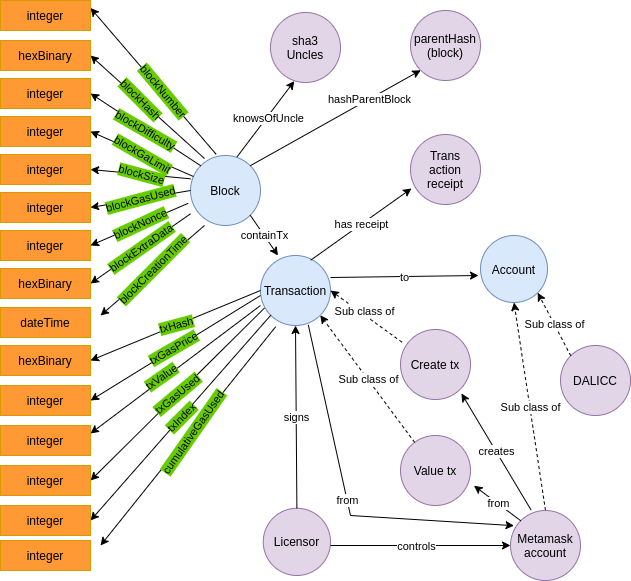
\includegraphics[width=1.45\textwidth]{images/chap03_knowledge_graph.png}
		\end{minipage}
		\caption{Transaction illustration}
		
	\end{figure}
	
\end{center}

\end{itemize}
\section{Project Architecture}

\subsection{Backend} The backend of this project relies on the Ethereum platform using smart contracts. In addition, DALICC license library the user can license here/his data or retrieve license information. In the next paragraph, we will more focused on authenticated users as the main challenge in decentralized apps and data licensing systems by users. \\
\\
\textbf{Authenticated user} \\
Authentication of users on Ethereum for validation purposes is the essential feature when building dApp.  Therefore, programming the functionality of Ethereum authentication for dApps is important for blockchain developers. 
In this dApp, we consider two solutions for Ethereum authentications as follows: \\
\\
\textit{- login to metamask:} Metamask is the most popular cryptocurrency wallet (Ethereum account) to support the Ethereum blockchain. Additionally, metamask is a bridge for web3 authentication to an Ethereum-based decentralized application. By logging into Metamsk, users can submit transactions or check the stored data on the blockchain.\\
\textit{- Using smart contract: } The address of the metamask is passed to smart contract as a licensor, then it will
use this address as an owner to license his/her file. \\
\\
\textbf{Licensing in smart contract} as follow: \\
\\
\textbf{License information} represents three elements: licensor address that is passed by metamask, license of data, and the URI related to this license.\\
\textbf{Storage license information}: Each smart contract that runs on the Ethereum blockchain would be maintained state in its permanent storage. The license information is stored in its storage and is changeable only by the smart contract itself.\\
\textbf{Retrieve license information}\\
As mentioned earlier, only a smart contract can change the data in its memory. Thus, we can consider smart contracts a validating system for license requests. The JavaScript
library web3.js is an interface to the Ethereum Network for the frontend of this dApp. This allows the frontend to access the smart contract, retrieving or changing license information.\\

\subsection{Frontend}
 Frontend of this project build on React.js, HTML, and CSS. The React js used in this front-end for the user interface.\\
 \\
 \textbf{User roadmap}\\
 The licensing Data from the user interface includes three phases:
 \begin{itemize}
 	\item The user gets asked to select to license type from which to be loaded from Dalicc Library via Axios and get a request in frontend. Then, after selecting data in the next field, the user should check the file, if the selected file is already licensed or not. Depending on this verification, the user receives either the confirmation message 'License detected' or the rejection message 'License not detected'. 
 	\item The user should go further by pressing the 'License Data/ retrieve license' button to get license information for the confirmation message of the last phase or license his/her file.\\
 License information contains some information like license type, license URI retrieved from the DALICC library, and the address of the owner of this license. For licensing data, the user gets asked to log in to Metamask for the authentication process and this address would be passed to smart contract as owner of this license. The licensing process will be done by receiving the hash value of licensed data.
 	\item In the last phase, the user can observe receipt of this transaction in a table that contains transaction details from the interaction between \textit{web3.eth} and \textit{ethOn ontology}.
 \end{itemize}
 \begin{center}
 	
 	\begin{figure}[htb!]
 		
 		\begin{minipage}{0.75\linewidth}
 			
 			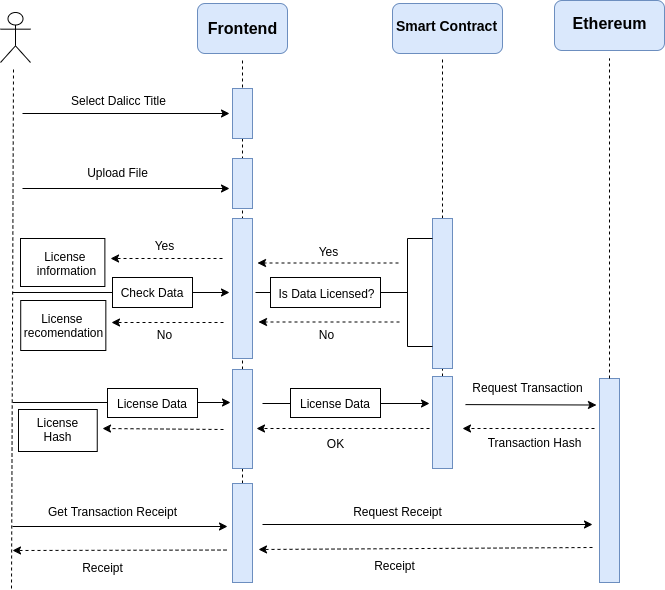
\includegraphics[width=1.45\textwidth]{images/chap03_user_roadmap.png}
 		\end{minipage}
 		\caption{Sequence diagram for licensing file}
  	\end{figure}
  \end{center}
 \textbf{Interaction with backend}\\
 Since the backend code(smart contract) of the dApp is on a decentralized network, we focused on the interaction between the smart contract and the Ethereum network. The communication between the fronted and backend is taken over by Java Script library \textit{web3.js}.
 For this purpose, web3 provides this connection either with HDWallet-provider to connect to the test network (Sepolia in our case) or Ethereum provider.\\
 \\
 \textbf{Interaction with with DALICC} \\
 To retrieve the license, an HTTP GET request is sent to the DALICC library endpoint and returns the license which encompasses two elements: license title and license URI. The user can choose just the DALICC title as a license then the URI of the associated title would be stored subsequently in the smart contract for further processing. \\
 \\
\textbf{License receipts}\\
After committing a transaction in the blockchain, the user can get transaction details via web.eth, then send transaction details in RDF format to the server to store into a file. The produced turtle file will be resulted into a readable format and would be returned to frontend by HTTP GET request from frontend.
\\
\subsection{DApp Architecture} 
This application encompasses some components:
\begin{itemize}
	\item User interface
	\item Smart contract to communicate with DALICC library
	\item Ethereum network to support transaction
	\item Transaction receipt
	\item EthOn ontology
	\item SPARQL query    
\end{itemize} 
\begin{center}
   \begin{figure}[htb!]
		
		\begin{minipage}{0.75\linewidth}
			
			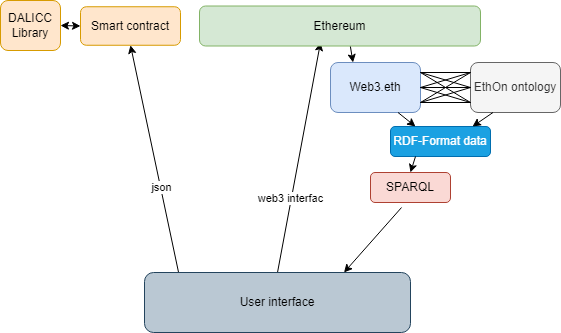
\includegraphics[width=1.5\textwidth]{images/chap03_eth_dalicc_comm.png}
		\end{minipage}
		\caption{DApp Architecture}
	\end{figure}
\end{center}

\section{Implementation}
This section comprises the implementation details in a smart contract and some main functions in the application.

\subsection{Smart Contract Logic}
As mentioned before, the backend code of this application is on the Ethereum network. in this section, we will contemplate more on each functionality of the contract in this dApp.
\begin{itemize}
	\item \textit{Owned contract} \\
	This smart contract contains the function to prevent non-owner users to call the function and the owner as the constructor to be usable in every contract which is called to. This contract provides a function that helps us to restrict access to some function in another contract that would be called later by them. \\
	\item \textit{PrimaryLicenseContract} \\
	This is the main contract that communicates with two other contracts to represent the public interface of the licensing system. It provides functions to licensing data or retrieves license information. \\
   \item \textit{LicenseManager contract} \\
	This smart contract is responsible for saving the address of the license or creating one for the new file. \\
	\item \textit{License contract} \\
	In this contract, the hash value and licensor address would be stored here. License contracts represent only one license and associate license contract for this license. The license contract should have been created by the license manager.

\end{itemize}

\begin{center}
	
	\begin{figure}[htb!]
		
		\begin{minipage}{0.75\linewidth}
			
			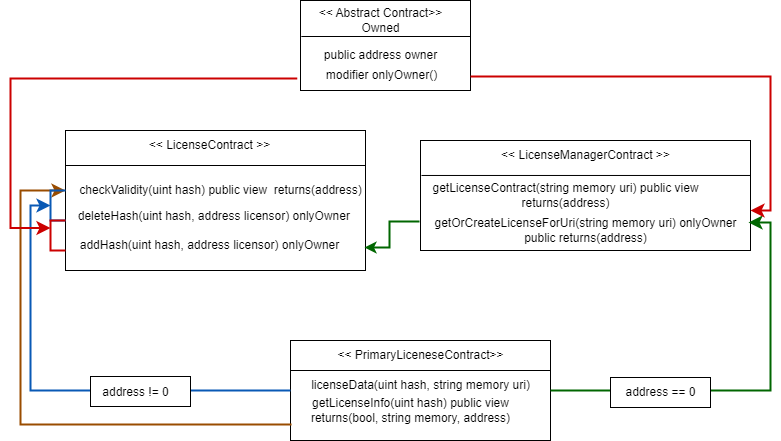
\includegraphics[width=1.45\textwidth]{images/chap03_smartContract_visual.png}
		\end{minipage}
		\caption{Smart contract visualization}
		
	\end{figure}
	
\end{center}

\text{How Smart Contract works?}

\begin{itemize}
	\item \textbf{Licensing system process} \\
	To license data, two parameters are needed. The first one is the hash of related data and the second one is the address related to the URI of the license. This smart contract as a \textit{caller} take over the process: \\
	\textbf{License data} \\
	To license data, the function \textit{licenseData} is used which declares with two parameters: the first one is the hash associated with selected data, and the second one is the URI of the selected license. By pressing the 'License Data/retrieve license on the frontend, the function
	\textit{licenseData} would be triggered and perform the steps as follow: \\
	This function checks if the target address is the zero account, which means the transaction creates a new contract: 
	if no, function \textit{deleteHash}, otherwise \textit{getOrCreateLicenseForUri} would be called. How does licensing data work? \\
	\begin{itemize}
		\item \textit{licenseData} function check if the specified hash is linked to a license and the caller is licensor, then \textit{deleteHash} is called and the hash of related data and address of licensor would be passed. \\
		\hspace{1cm} \textbf{Definition} \textit{deleteHash}: This function is accessible just for the owner (function caller), which means the caller of this function must be the owner and the passed address should be the licensor. Then the link between the hash and license will be dropped.
		\item \textit{getOrCreateLicenseForUri} of the license Manager is called and the URI of the selected data as input parameter would be passed and returns the address to license contract which represents this URI.\\
		\hspace{1cm} \textbf{Definition} \textit{getOrCreateLicenseForUri}: This function checks if the caller of this function is the owner, then exists a license contract for a given URI. If so, the address of this license contract would be returned. Otherwise, a new license contract will be created and the address of the contract will be stored and returned. The caller's address of the caller also will be used later as the owner of this contract.
		\item \textit{addHash} function of the License contract is called with two parameters: the first one if the hash of data, and the second one is the function caller.\\
		\hspace{1cm} \textbf{Definition} \textit{addHash}: This function is accessible just for the owner (function caller), the link between the hash value and the license is created. The second parameter would be stored also as licensor. \\
		\item At the end, the event should be emitted to fire the new changes in PrimaryLicenseContarct.
		
	\end{itemize}
	\item \textbf{Change license data} \\
	This is doable just by the licensor in the same way as license data.  \\
	\item \textbf{Retrieve license information} \\
	To retrieve license information function \textit{getLicenseInfo} is called having a hash of data as a parameter and checks if there is some license information related to this hash, then is returned the address otherwise, returns a null address and string.
	
\end{itemize}
\subsection{Forntend Workflow}
\begin{itemize}
	\item Define type:
	In this step, the user gets asked to select a license type among many different licenses. These licenses are loaded from DALICC License Library via \textit{axios} GET request. And user must choose one of them to continue license processing.
 \begin{center}
	\begin{figure}[htb!]
		
		\begin{minipage}{0.45\linewidth}
			\centering
			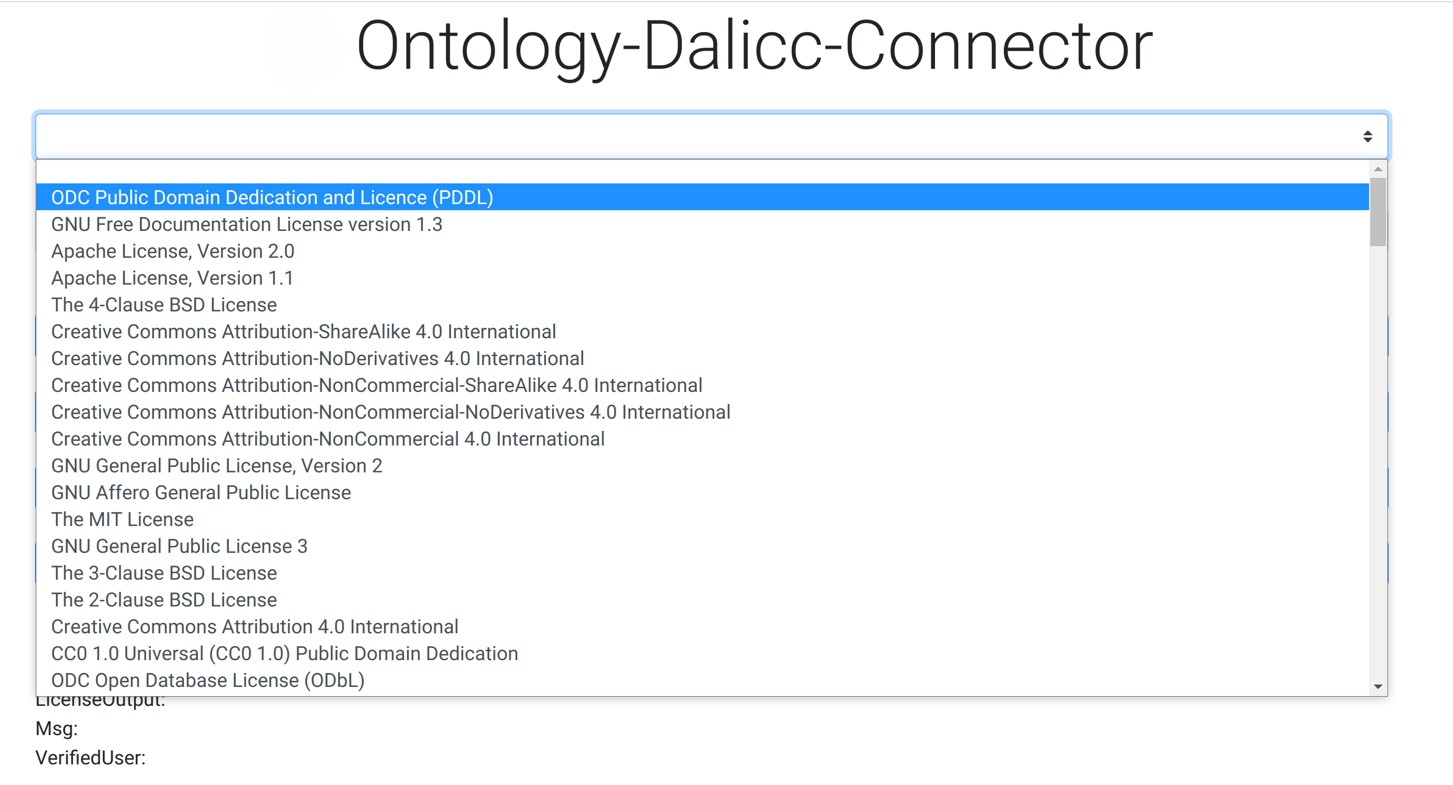
\includegraphics[width=1.95\textwidth]{images/chap03_selectType.jpg}
		\end{minipage}
		\caption[Define Type from DALICC library]{Define Type from DALICC library}
		
	\end{figure}
	
\end{center}
	\item Define Content:
	In this step, the user should choose the file or data that wants to be licensed. Subsequently, the hash \texttt{SHA3-256} of the selected file is calculated which is used to retrieve license information later.
 \begin{center}
	\begin{figure}[htb!]
		
		\begin{minipage}{0.45\linewidth}
			\centering
			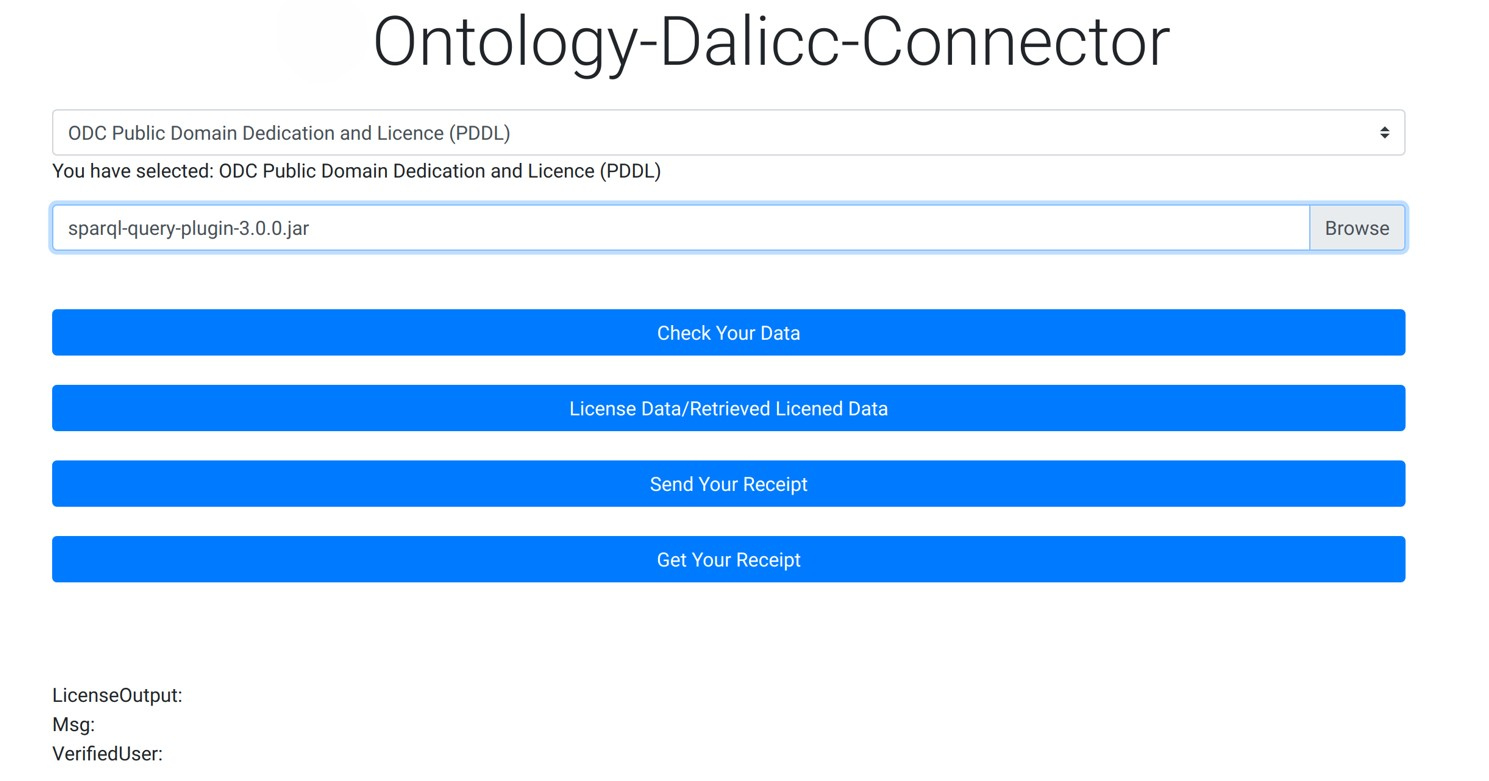
\includegraphics[width=1.95\textwidth]{images/chap03_selectFile.jpg}
		\end{minipage}
		\caption[Define file from local device]{Define file from local device}
		
	\end{figure}
\end{center}
	\item Check Your Data:
	In this step, the user should check the selected data: if it is licensed before or not. He/ she receives just a message either confirmation 'License is detected' or rejection 'License is not detected'. He or she should go further to obtain more information.
    \begin{center}
	\begin{figure}[htb!]
		
		\begin{minipage}{0.45\linewidth}
			\centering
			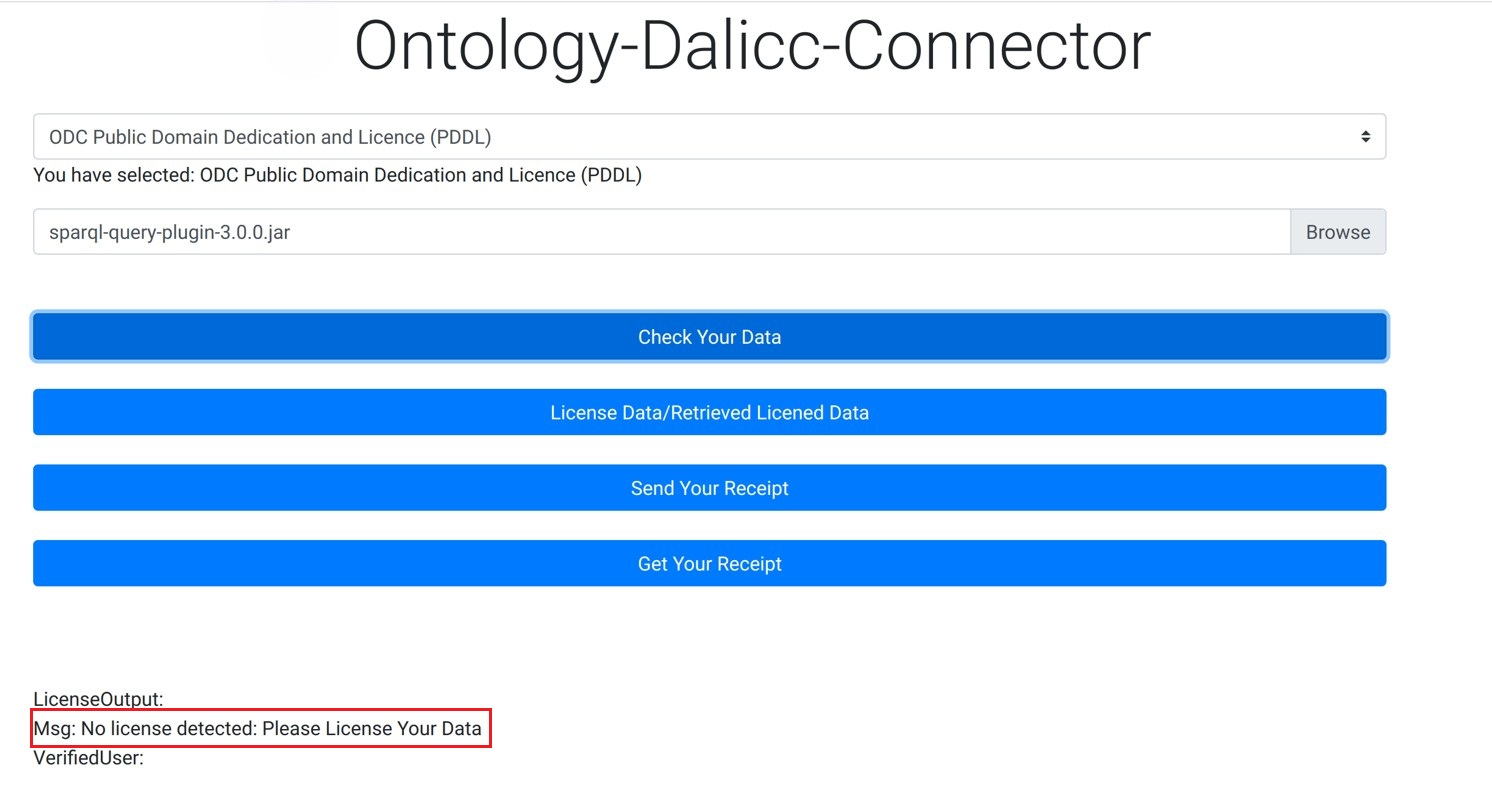
\includegraphics[width=1.95\textwidth]{images/chap03_checkFile.jpg}
		\end{minipage}
		\caption[Check if file is already licensed?]{Check if file is already licensed?}
		
	\end{figure}
	
\end{center}

\begin{center}
	\begin{figure}[htb!]
		
		\begin{minipage}{0.45\linewidth}
			\centering
			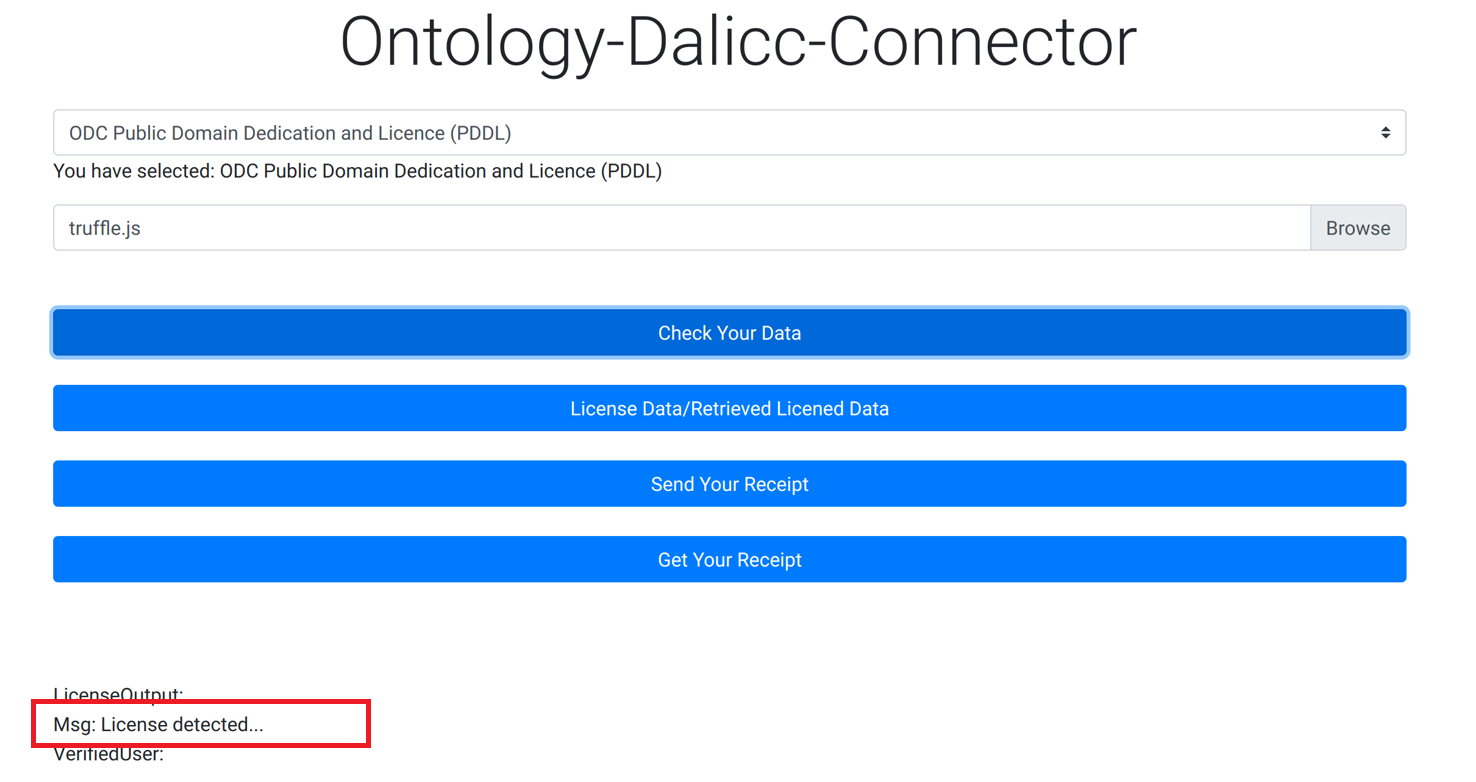
\includegraphics[width=1.95\textwidth]{images/chap03_found_license.png}
		\end{minipage}
		\caption[message for licensed data]{message for licensed data}
		
	\end{figure}
	
\end{center}
	\item License data / retrieve License information:
	Here, the user receives the result of that last step, by pressing the hash value of selected data \texttt{SHA3-256} is calculated and passed to the smart contract using \textit{web. js} interface: \\
    \\
	\textbf{- } License information of the selected file or data from which the user received the 'license detected' message from the last step. The user receives some information related to the license, licensor address, and URI related to the license.\\
    \begin{center}
	\begin{figure}[htb!]
		
		\begin{minipage}{0.55\linewidth}
			\centering
			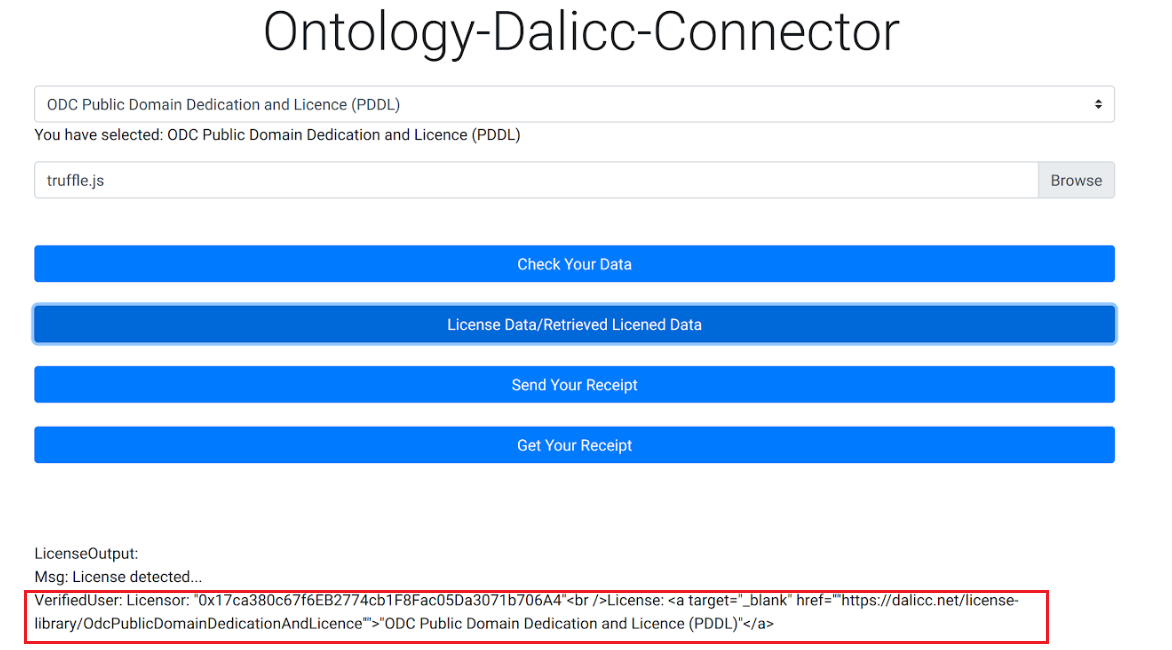
\includegraphics[width=1.95\textwidth]{images/chap03_found_info.png}
		\end{minipage}
		\caption[license information for already licensed data]{license information for already licensed data}
		
	\end{figure}
	
\end{center}
    \textbf{- } Start licensing he/her file, if he/she received 'No license detected'  from the last step. To license data, the user gets asked to log into \texttt{Metamask} to pass this account as the address of the licensor to the smart contract. The SHA3-256 hash value is calculated and passed by the contract to the Web3 Javascript interface. Users can see this hash in the front end, depending on the successful transaction or he/she receives the error message for failed transaction on the front end.\\
    \begin{center}
	 \begin{figure}[htb!]
		\begin{minipage}{0.45\linewidth}
			\centering
			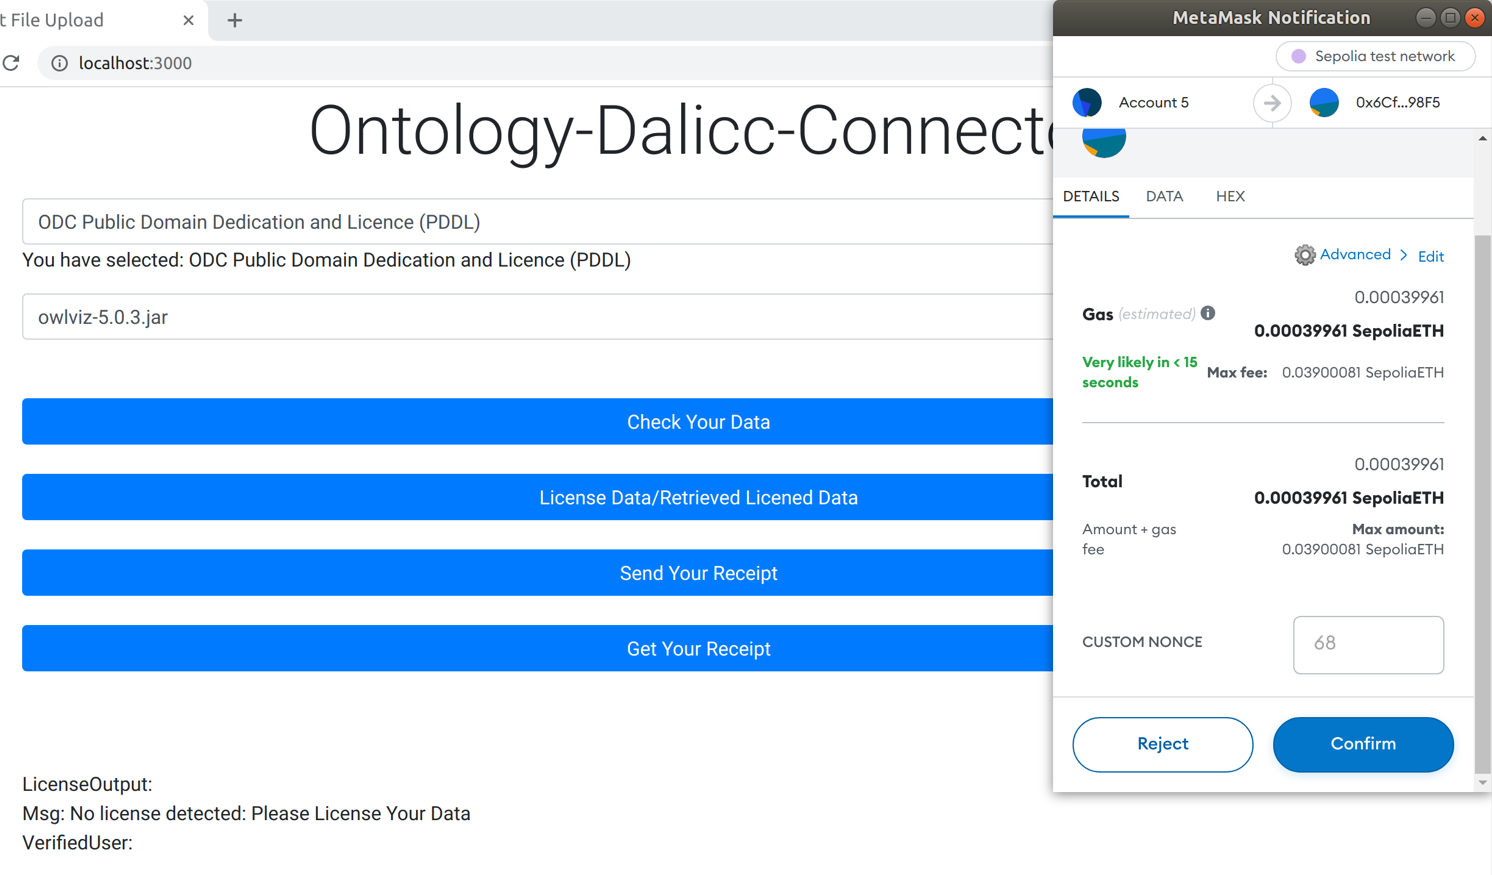
\includegraphics[width=1.95\textwidth]{images/chap03_license_data.png}
		\end{minipage}
		\caption[licensing data process]{licensing data process}
		
	\end{figure}
\end{center}
   \begin{center}
	\begin{figure}[htb!]
		
		\begin{minipage}{0.45\linewidth}
			\centering
			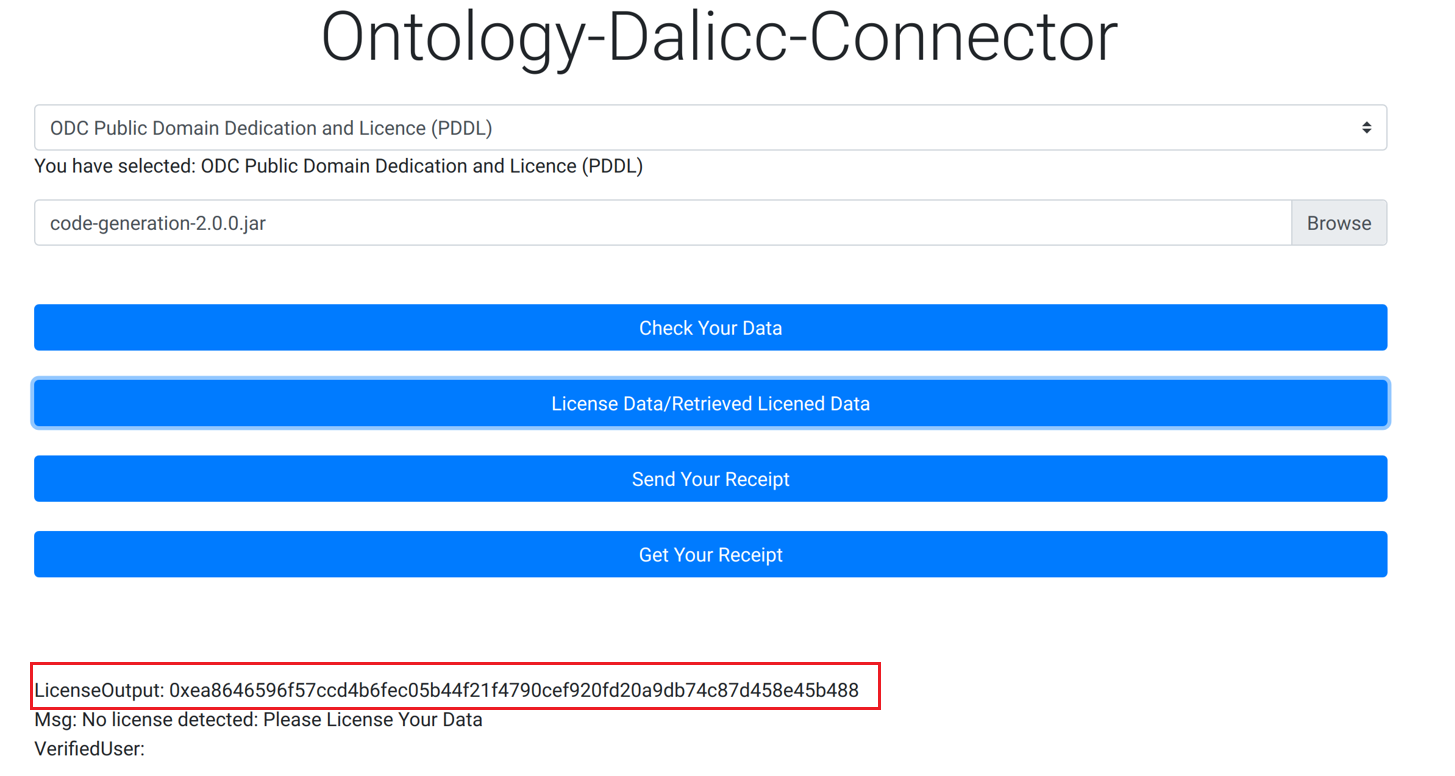
\includegraphics[width=1.95\textwidth]{images/chap03_license_hash.png}
		\end{minipage}
		\caption[License hash after confirming transaction]{License hash after confirming transaction}
		
	\end{figure}
\end{center}
   

\begin{center}
	\begin{figure}[htb!]
		
		\begin{minipage}{0.45\linewidth}
			\centering
			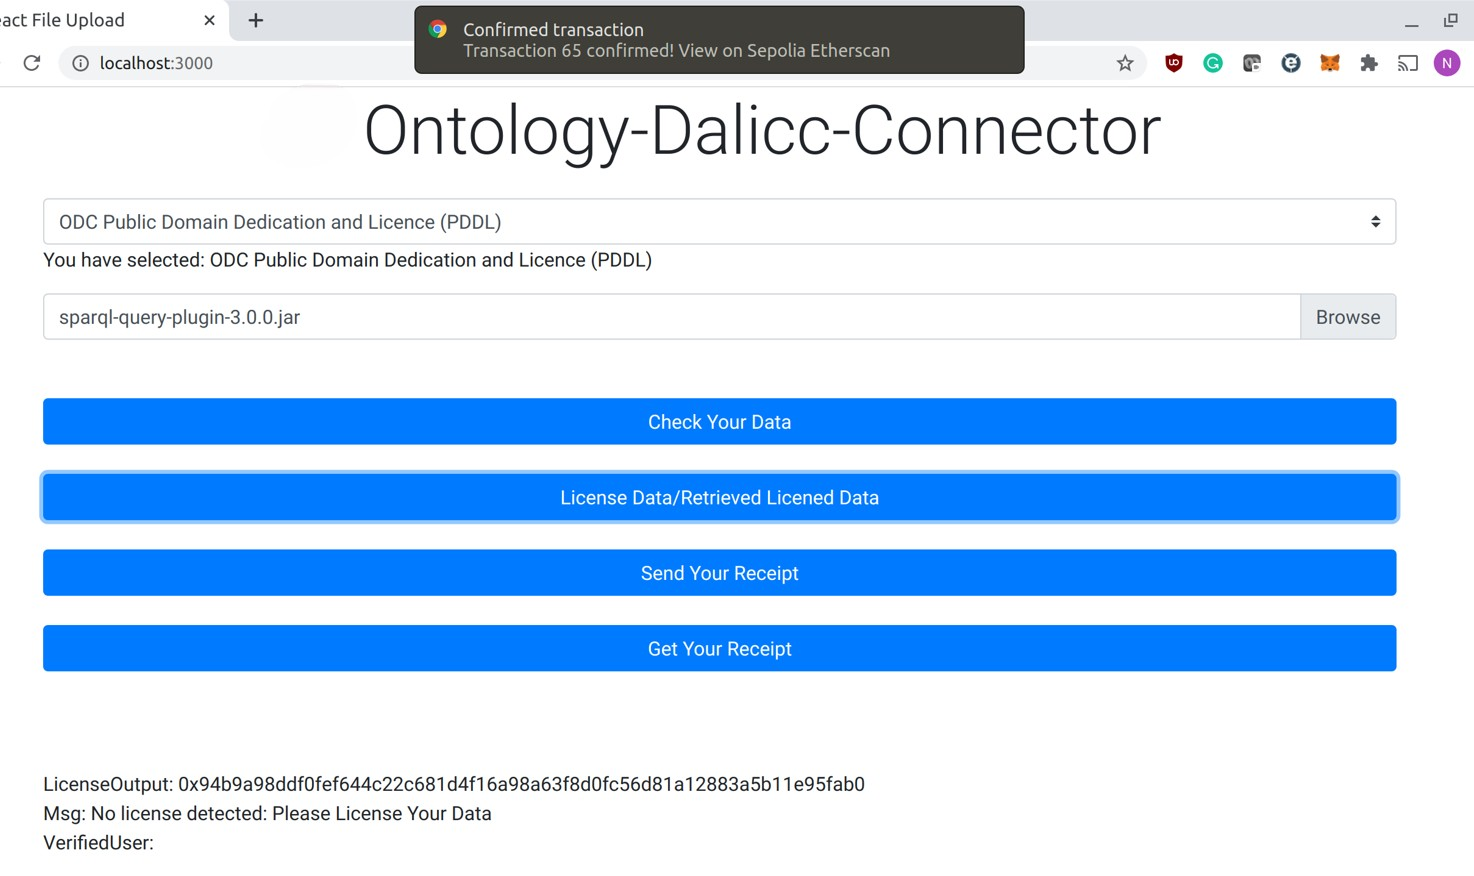
\includegraphics[width=1.95\textwidth]{images/chap03_confirm_tx.jpg}
		\end{minipage}
		\caption[Transaction confirmation]{Transaction confirmation}
		
	\end{figure}
	
\end{center}
	\item Send transaction: After receiving the hash of the transaction in the frontend, the user goes further to get a receipt of this licensing having all details about the transaction. to have this receipt user sends a transaction receipt that is not readable to the server for more processing on this raw result, converting to RDF format data and making a query to produce more readable RDF-based data.
	\item Get Transaction receipt:
	In the last step, the user can get a receipt of all transactions that have been done till now as a table in RDF format.
\end{itemize}

\begin{center}
	\begin{figure}[htb!]
		
		\begin{minipage}{0.55\linewidth}
			\centering
			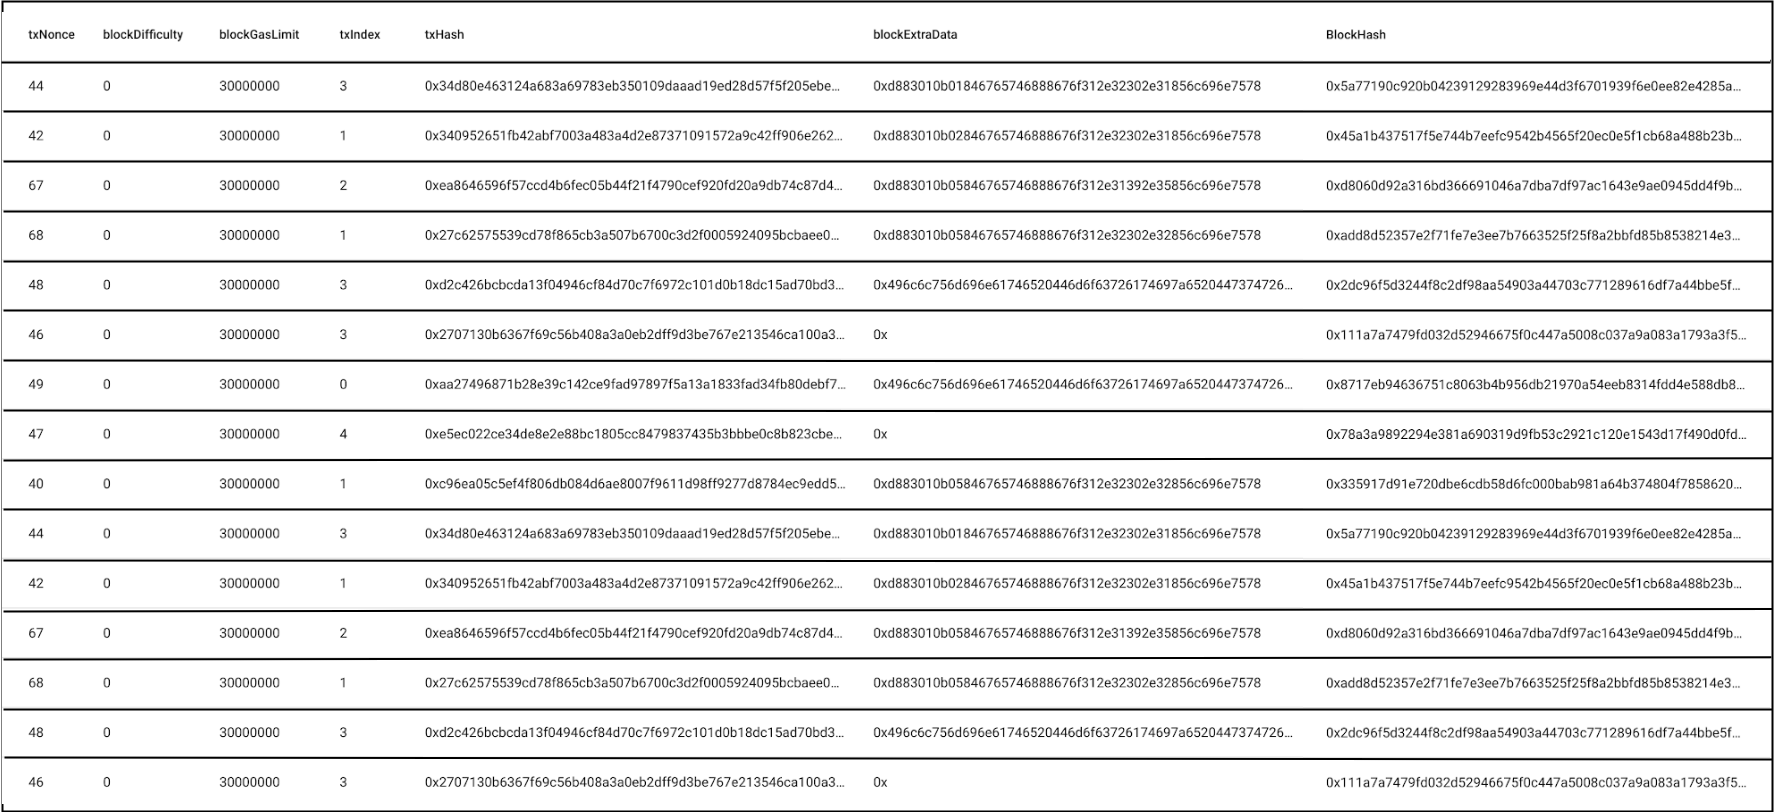
\includegraphics[width=1.95\textwidth]{images/chap03_licese_result_1.png}
		\end{minipage}
		\caption[Result of semantic mapping]{Result of semantic mapping}
		
	\end{figure}
	
\end{center}
\begin{center}
	\begin{figure}[htb!]
		
		\begin{minipage}{0.55\linewidth}
			\centering
			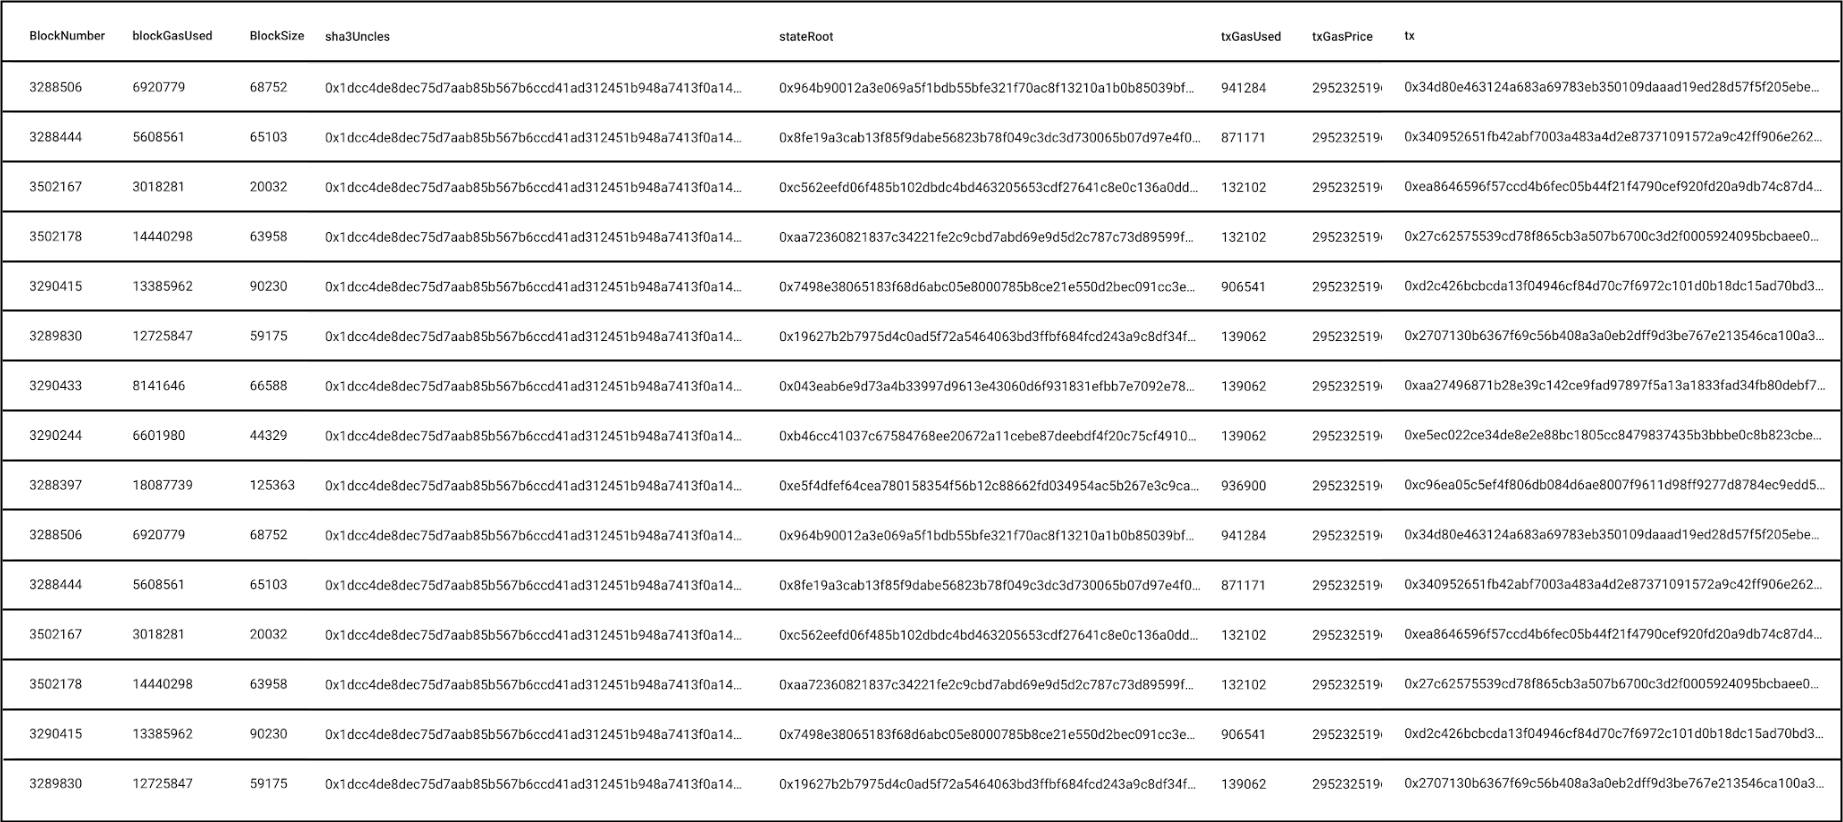
\includegraphics[width=1.95\textwidth]{images/chap03_licese_result_2.png}
		\end{minipage}
		\caption[Result of semantic mapping]{Result of semantic mapping}
		
	\end{figure}
	
\end{center}
\chapter{Conclusion}
In this work, we attempted to analyze smart contract and their integration with semantic web data licesing. To achieve this goal, first we tried to analyze blockchain where smart contract reside on it as program code. Afterwards, we showed that how blockchain could be applied as computational paradigm for semantic web and linked data. Then we focused on bitcoin, Etheruem as main usage of blockahin and related vulnerabilities in Ethereum.
Furthermore, we have presented the first initial effort to use this construct in useful ways by extending blockchain with semantic web in supply chain management. As the main goal of this work is to show ssemantic web principle can be use in making smarter smart contract and blockchain network. First, we started presenting our work done in ontology, Ethereum ontology (EthOn) describes blockchain structure and related information such as classes, object properties and etc. Later, we used this concept as RDF triple format which will feed by dataset and will lead into representing our data based on query.

%now enable appendix numbering format and include any appendices
\appendix
\chapter{Semantic mapping column in web3}
The appendix comprises semantic mapping elements described and the source code for the smart contracts described in forth  chapter.
\small

\begin{center}
	\begin{figure}[htb!]
		
		\begin{minipage}{0.15\textwidth}
           \centering
			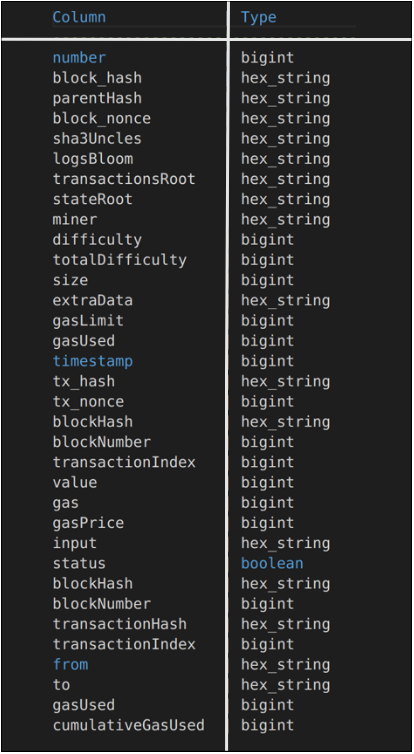
\includegraphics[width=1.95\textwidth]{images/chap03_web3_schema.png}
		\end{minipage}
	
	\end{figure}
	
\end{center}
\chapter{RDF triple template in semantic mapping }
\begin{center}
	\begin{figure}[htb!]
		
		\begin{minipage}{0.43\linewidth}
			\centering
			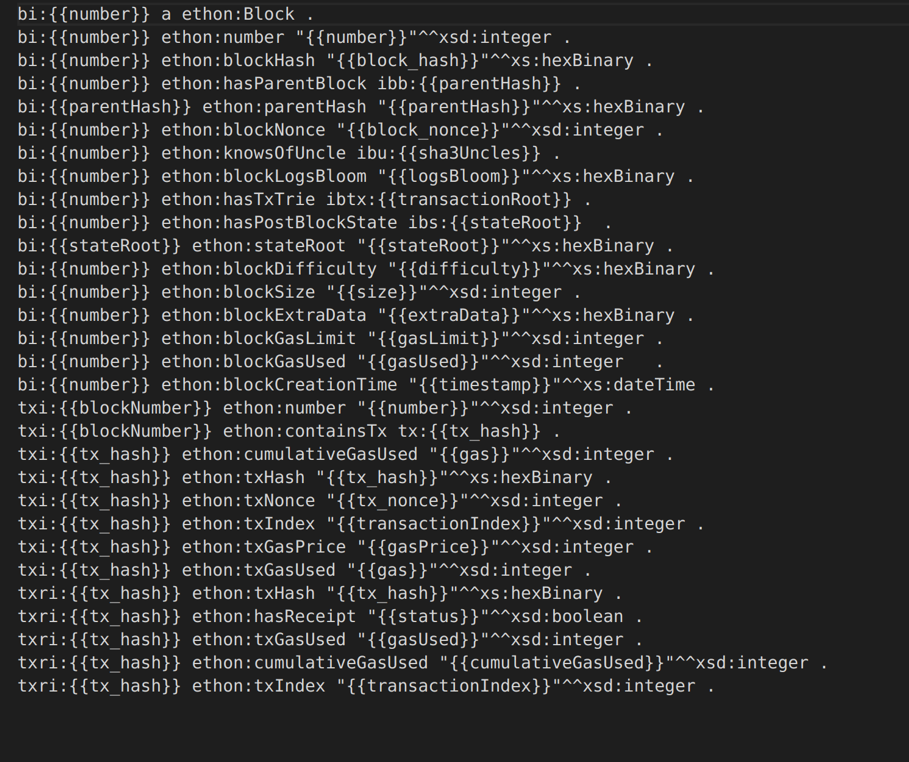
\includegraphics[width=1.95\textwidth]{images/chap03_triple_template.png}
		\end{minipage}
		
	\end{figure}
	
\end{center}

\chapter{Tripleize application}
\small
\vspace{0.2in}
\begin{lstlisting}
@prefix ethon: <http://ethon.consensys.net/> .
@prefix ibb: <http://ethon.consensys.net/Block#> .
@prefix ibu: <http://ethon.consensys.net/Uncle#> .
@prefix ibs: <http://ethon.consensys.net/State#> .
@prefix tx: <http://ethon.consensys.net/Tx#> .
@prefix xsd: <http://www.w3.org/2001/XMLSchema#> .



ibb:10192431 ethon:containsTx tx:0x33e7b8e4b0d968f916429c39416dc61e1838dd4c0868929ca2aff1de196d63fb .

tx:0x33e7b8e4b0d968f916429c39416dc61e1838dd4c0868929ca2aff1de196d63fb  ethon:number "10192431"^^xsd:hexBinary .

tx:0x33e7b8e4b0d968f916429c39416dc61e1838dd4c0868929ca2aff1de196d63fb  ethon:blockCreationTime "2020-06-03 10:56:19"^^xsd:dateTime .

tx:0x33e7b8e4b0d968f916429c39416dc61e1838dd4c0868929ca2aff1de196d63fb  ethon:from "0xd551234ae421e3bcba99a0da6d736074f22192ff"^^xsd:hexBinary .

tx:0x33e7b8e4b0d968f916429c39416dc61e1838dd4c0868929ca2aff1de196d63fb  ethon:to "0x61c808d82a3ac53231750dadc13c777b59310bd9"^^xsd:hexBinary .

tx:0x33e7b8e4b0d968f916429c39416dc61e1838dd4c0868929ca2aff1de196d63fb  ethon:address ""^^xsd:hexBinary .

tx:0x33e7b8e4b0d968f916429c39416dc61e1838dd4c0868929ca2aff1de196d63fb  ethon:txGasPrice  "10000"^^xsd:integer .

tx:0x33e7b8e4b0d968f916429c39416dc61e1838dd4c0868929ca2aff1de196d63fb  ethon:txGasUsed  "0"^^xsd:integer .

tx:0x33e7b8e4b0d968f916429c39416dc61e1838dd4c0868929ca2aff1de196d63fb  ethon:ValueTx  "2365900"^^xsd:integer .





ibb:9235119 ethon:containsTx tx:0x6bc23e9a66cda5e4052e55658836286094f22a214b014c7fd3c238b1f76ce170 .

tx:0x6bc23e9a66cda5e4052e55658836286094f22a214b014c7fd3c238b1f76ce170  ethon:number "9235119"^^xsd:hexBinary .

tx:0x6bc23e9a66cda5e4052e55658836286094f22a214b014c7fd3c238b1f76ce170  ethon:blockCreationTime "2020-01-07 18:25:58"^^xsd:dateTime .

tx:0x6bc23e9a66cda5e4052e55658836286094f22a214b014c7fd3c238b1f76ce170  ethon:from "0x876eabf441b2ee5b5b0554fd502a8e0600950cfa"^^xsd:hexBinary .

tx:0x6bc23e9a66cda5e4052e55658836286094f22a214b014c7fd3c238b1f76ce170  ethon:to "0x61c808d82a3ac53231750dadc13c777b59310bd9"^^xsd:hexBinary .

tx:0x6bc23e9a66cda5e4052e55658836286094f22a214b014c7fd3c238b1f76ce170  ethon:address ""^^xsd:hexBinary .

tx:0x6bc23e9a66cda5e4052e55658836286094f22a214b014c7fd3c238b1f76ce170  ethon:txGasPrice  "12.08883888"^^xsd:integer .

tx:0x6bc23e9a66cda5e4052e55658836286094f22a214b014c7fd3c238b1f76ce170  ethon:txGasUsed  "0"^^xsd:integer .

tx:0x6bc23e9a66cda5e4052e55658836286094f22a214b014c7fd3c238b1f76ce170  ethon:ValueTx  "2860.0983906192"^^xsd:integer .





ibb:9311763 ethon:containsTx tx:0xb5b345ed7ebd23c903023dad437fd62046a80416c36b0604dd09e71aa245b9dc .

tx:0xb5b345ed7ebd23c903023dad437fd62046a80416c36b0604dd09e71aa245b9dc  ethon:number "9311763"^^xsd:hexBinary .

tx:0xb5b345ed7ebd23c903023dad437fd62046a80416c36b0604dd09e71aa245b9dc  ethon:blockCreationTime "2020-01-19 12:28:07"^^xsd:dateTime .

tx:0xb5b345ed7ebd23c903023dad437fd62046a80416c36b0604dd09e71aa245b9dc  ethon:from "0x61c808d82a3ac53231750dadc13c777b59310bd9"^^xsd:hexBinary .

tx:0xb5b345ed7ebd23c903023dad437fd62046a80416c36b0604dd09e71aa245b9dc  ethon:to "0xdac17f958d2ee523a2206206994597c13d831ec7"^^xsd:hexBinary .

tx:0xb5b345ed7ebd23c903023dad437fd62046a80416c36b0604dd09e71aa245b9dc  ethon:address ""^^xsd:hexBinary .

tx:0xb5b345ed7ebd23c903023dad437fd62046a80416c36b0604dd09e71aa245b9dc  ethon:txGasPrice  "0"^^xsd:integer .

tx:0xb5b345ed7ebd23c903023dad437fd62046a80416c36b0604dd09e71aa245b9dc  ethon:txGasUsed  "0"^^xsd:integer .

tx:0xb5b345ed7ebd23c903023dad437fd62046a80416c36b0604dd09e71aa245b9dc  ethon:ValueTx  "0"^^xsd:integer .






ibb:9768545 ethon:containsTx tx:0x6db07c30c528dbe2bde5bf0487fbc6d379764b20390832546c665c7a09281ca0 .

tx:0x6db07c30c528dbe2bde5bf0487fbc6d379764b20390832546c665c7a09281ca0  ethon:number "9768545"^^xsd:hexBinary .

tx:0x6db07c30c528dbe2bde5bf0487fbc6d379764b20390832546c665c7a09281ca0  ethon:blockCreationTime "2020-03-29 19:50:21"^^xsd:dateTime .

tx:0x6db07c30c528dbe2bde5bf0487fbc6d379764b20390832546c665c7a09281ca0  ethon:from "0x876eabf441b2ee5b5b0554fd502a8e0600950cfa"^^xsd:hexBinary .

tx:0x6db07c30c528dbe2bde5bf0487fbc6d379764b20390832546c665c7a09281ca0  ethon:to "0x61c808d82a3ac53231750dadc13c777b59310bd9"^^xsd:hexBinary .

tx:0x6db07c30c528dbe2bde5bf0487fbc6d379764b20390832546c665c7a09281ca0  ethon:address ""^^xsd:hexBinary .

tx:0x6db07c30c528dbe2bde5bf0487fbc6d379764b20390832546c665c7a09281ca0  ethon:txGasPrice  "200.00041209"^^xsd:integer .

tx:0x6db07c30c528dbe2bde5bf0487fbc6d379764b20390832546c665c7a09281ca0  ethon:txGasUsed  "0"^^xsd:integer .

tx:0x6db07c30c528dbe2bde5bf0487fbc6d379764b20390832546c665c7a09281ca0  ethon:ValueTx  "47318.0974963731"^^xsd:integer .








\end{lstlisting}




\chapter{SPARQL query example}
\begin{center}
	\begin{figure}[htb!]
		
		\begin{minipage}{0.43\linewidth}
			\centering
			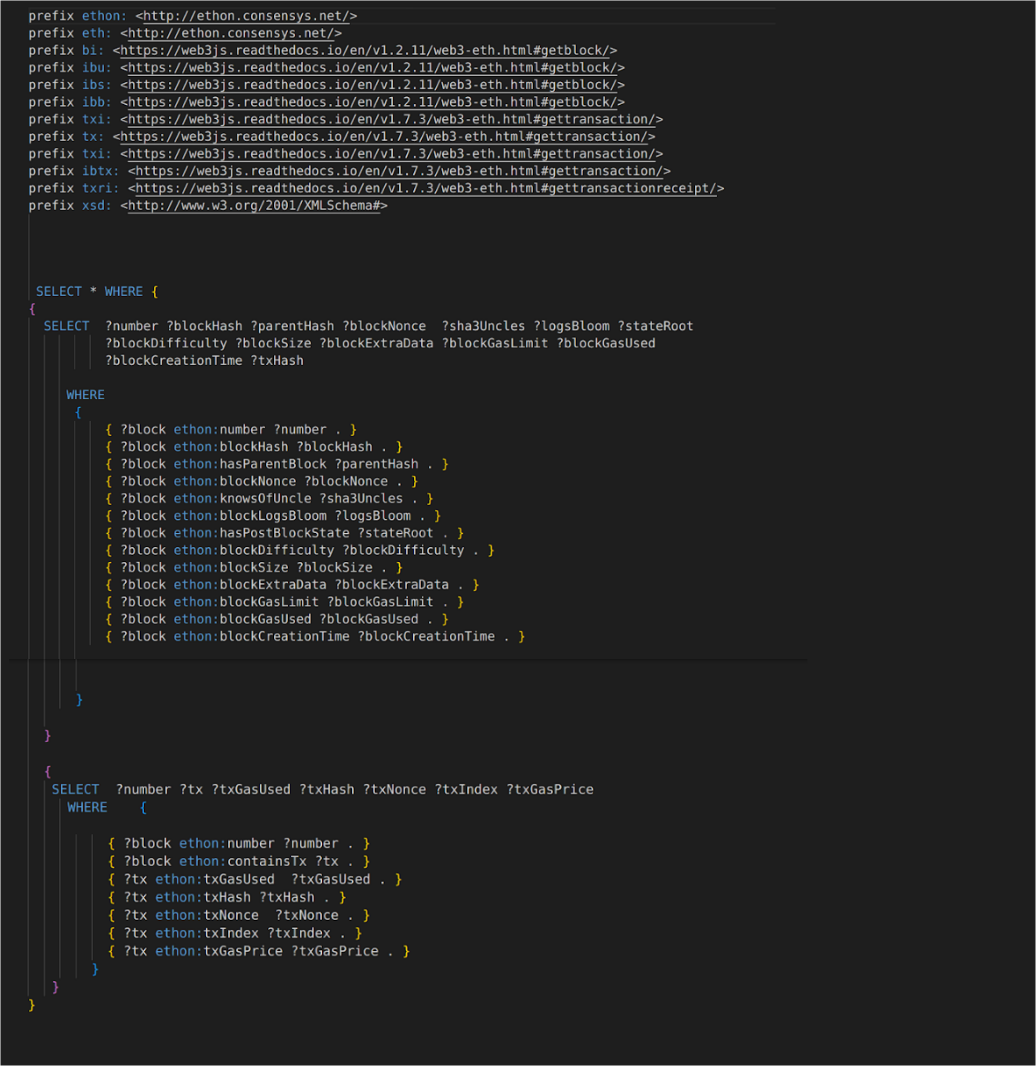
\includegraphics[width=1.95\textwidth]{images/chap03_sparql_query_2.png}
		\end{minipage}
		
	\end{figure}
	
\end{center}

\chapter{Smart contract}
\begin{center}
	\begin{figure}[htb!]
		
		\begin{minipage}{0.43\linewidth}
			\centering
			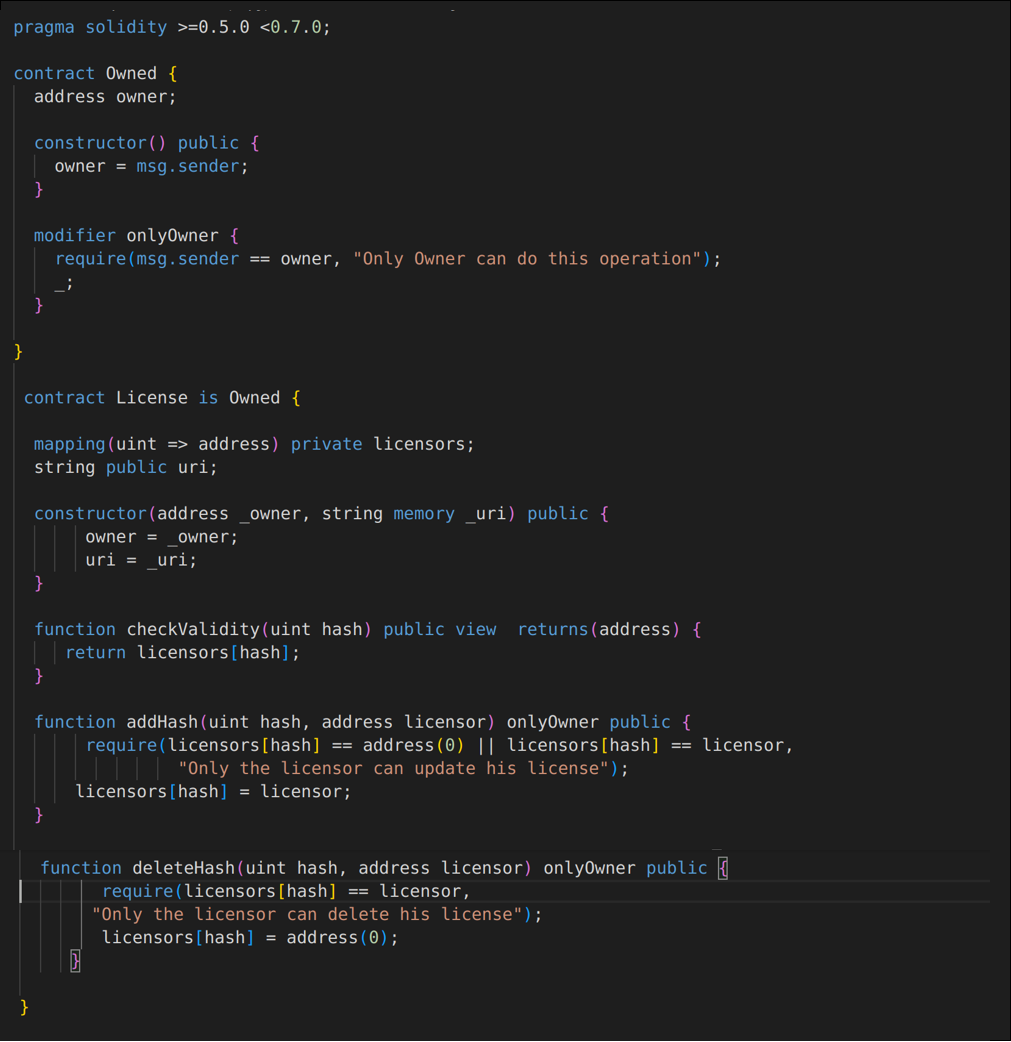
\includegraphics[width=1.95\textwidth]{images/chap03_sc_owner_license.png}
		\end{minipage}
		
	\end{figure}
	
\end{center}

\chapter{Smart contract}
\begin{center}
	\begin{figure}[htb!]
		
		\begin{minipage}{0.43\linewidth}
			\centering
			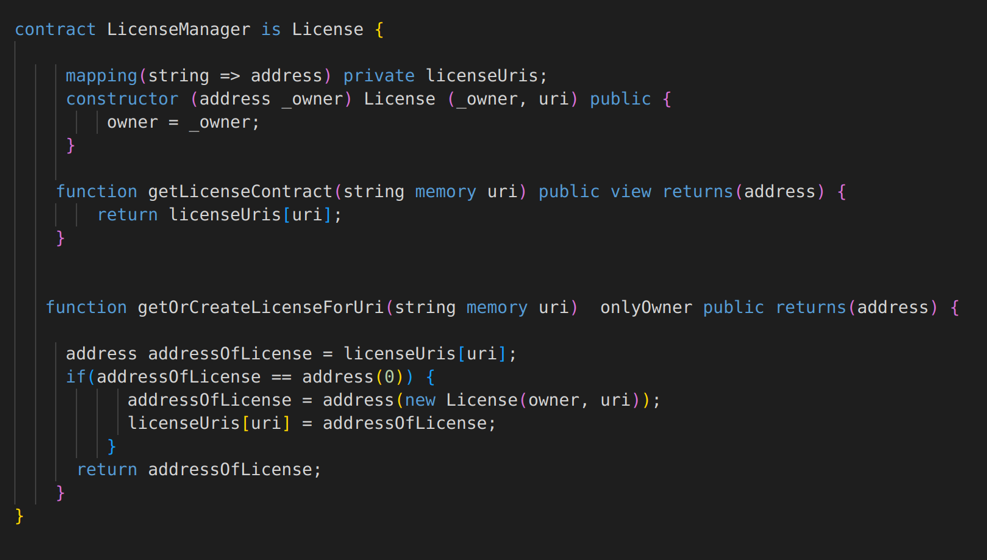
\includegraphics[width=1.95\textwidth]{images/chap03_sc_manager.png}
		\end{minipage}
		
	\end{figure}
	
\end{center}

\chapter{Smart contract}
\begin{center}
	\begin{figure}[htb!]
		
		\begin{minipage}{0.43\linewidth}
			\centering
			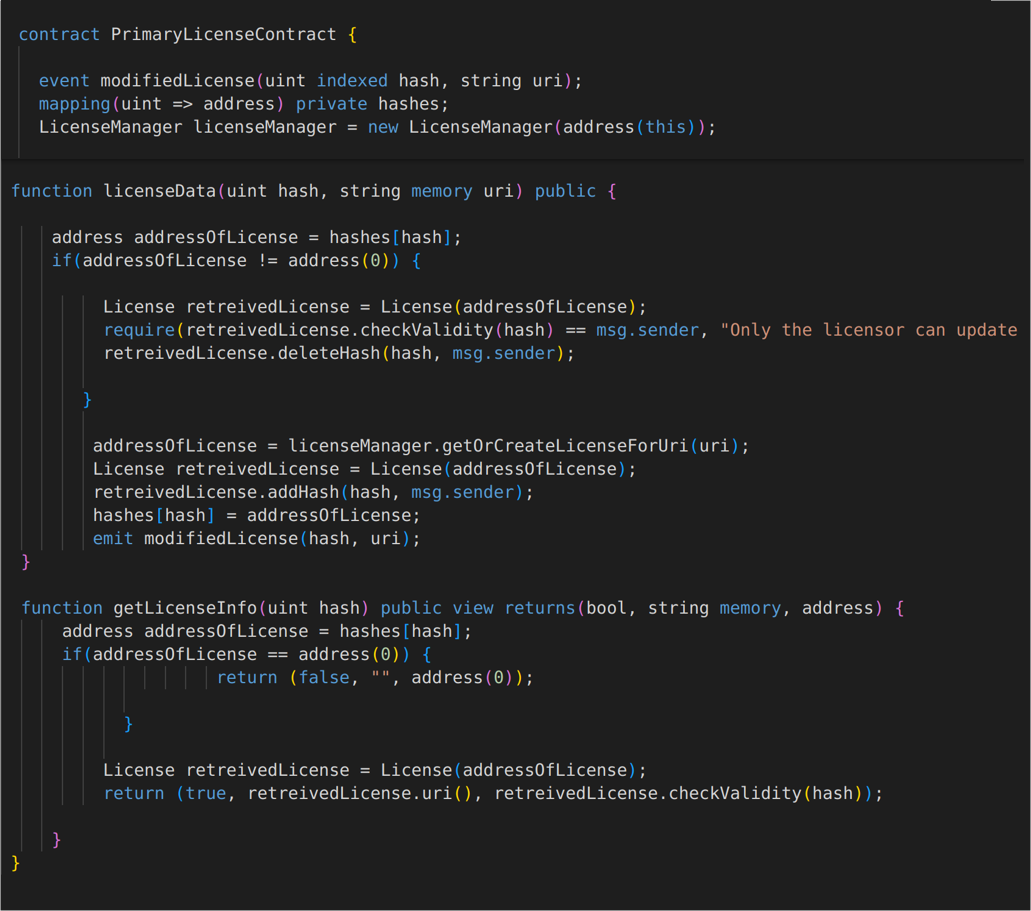
\includegraphics[width=1.95\textwidth]{images/chap03_sc_primary.png}
		\end{minipage}
		
	\end{figure}
	
\end{center}

\chapter{result of semantic mapping in RDF format}
\begin{center}
	\begin{figure}[htb!]
		
		\begin{minipage}{0.35\linewidth}
			\centering
			\includegraphics[width=1.95\textwidth]{images/chap03_triple_result.png}
		\end{minipage}
		
	\end{figure}
	
\end{center}
\bibliographystyle{apalike}
\bibliography{biblio}
%next line adds the Bibliography to the contents page
\addcontentsline{toc}{chapter}{Bibliography}
%uncomment next line to change bibliography name to references
%\renewcommand{\bibname}{References}
%\bibliography{refs.bib}        %use a bibtex bibliography file refs.bib
%\bibliographystyle{plain}  %use the plain bibliography style

\end{document}

